\documentclass[11pt, a4 paper]{article}
% Set target color model to RGB
\usepackage[inner=2.0cm,outer=2.0cm,top=2cm,bottom=2cm]{geometry}
\usepackage{setspace}
\usepackage{verbatim}
\usepackage{subcaption}
\usepackage{amsgen,amsmath,amstext,amsbsy,amsopn,tikz,amssymb}
\usepackage{fancyhdr}
\usepackage[colorlinks=true, urlcolor=blue,  linkcolor=blue, citecolor=blue]{hyperref}
\usepackage{subcaption}
\usepackage{sectsty}
\hypersetup{%
pdfauthor={Abijith J Kamath},%
pdftitle={Homework},%
pdfkeywords={Tikz,latex,bootstrap,uncertaintes},%
pdfcreator={PDFLaTeX},%
pdfproducer={PDFLaTeX},%
}

\newcommand{\ra}[1]{\renewcommand{\arraystretch}{#1}}

\newtheorem{thm}{Theorem}[section]
\newtheorem{prop}[thm]{Proposition}
\newtheorem{lem}[thm]{Lemma}
\newtheorem{cor}[thm]{Corollary}
\newtheorem{defn}[thm]{Definition}
\newtheorem{rem}[thm]{Remark}
\numberwithin{equation}{section}

\newcommand{\homework}[6]{
   \pagestyle{myheadings}
   \thispagestyle{plain}
   \newpage
   \setcounter{page}{1}
   \noindent
   \begin{center}
   \framebox{
      \vbox{\vspace{2mm}
    \hbox to 6.28in { {\bf E1 213:~Pattern Recognition and Neural Networks\hfill {\small Spring 2021}} }
       \vspace{6mm}
       \hbox to 6.28in { {\bfseries \Large \hfill #1  \hfill} }
       \vspace{6mm}
       \hbox to 6.28in { {\it Author: {\rm Abijith J. Kamath}} \hfill {\small {\it Email:} abijithj@iisc.ac.in}}
      \vspace{2mm}}
   }
   \end{center}
   \markboth{E1 213 -- #1}{E1 213 -- #1}
   \vspace*{4mm}
}

\newcommand{\problem}[1]{~\\\fbox{\textbf{#1}}\newline\newline}
\newcommand{\subproblem}[1]{~\newline\textbf{(#1)}}

\newcommand{\solution}{~\newline\textbf{\textit{(Solution)}} }

\linespread{1.3}

\setlength{\intextsep}{20pt} % Vertical space above & below [h] floats
\setlength{\textfloatsep}{20pt} % Vertical space below (above) [t] ([b]) floats
\setlength{\abovecaptionskip}{10pt}
\setlength{\belowcaptionskip}{10pt}

\newcommand{\by}{\mathbf{y}}
\newcommand{\bx}{\mathbf{x}}
\newcommand{\bX}{\mathbf{X}}
\newcommand{\bW}{\mathbf{W}}
\newcommand{\bA}{\mathbf{A}}
\newcommand{\bF}{\mathbf{F}}
\newcommand{\rr}{\mathbb{R}}
\newcommand{\cc}{\mathbb{C}}
\newcommand{\Ex}{\mathbb{E}}
\newcommand{\TT}{\mathsf{T}}
\newcommand{\HH}{\mathsf{H}}

\newcommand{\bmu}{\boldsymbol{\mu}}
\newcommand{\bSigma}{\boldsymbol{\Sigma}}

\chapterfont{\fontfamily{lmss}\selectfont}
\sectionfont{\fontfamily{lmss}\selectfont}
\subsectionfont{\fontfamily{lmss}\selectfont}

\begin{document}
\homework{1 : Implementing Bayes' Classifier}{}




\section*{Introduction}
\label{sec:intro}

Let patterns be in $\rr^d$ and consider the $2$-class classification problem -- given a pattern $\bx$, classify the pattern into a class with label $y$. In Bayesian classification theory, the training data $\{\bx^{(i)}, y^{(i)}\}_{i=1}^n$ is viewed to be i.i.d samples of the random vector $(\bX, Y)$. The training samples are used to model the joint distribution of the random vector $(\bX, Y)$.

Let $\Pr(C_i) = p_i$ be the priors associated with the $i$th class, $i=0,1$; and let $f_i(\bx) = p_{\bX\vert Y}(\bx \vert y=i)$ be the class-conditional densities. Using the Bayes' rule and the training data, the update on the probabilities of the classes as:
\begin{equation}
	q_i(\bx) = \Pr(y=i\vert \bX=\bx) = \frac{p_{\bX\vert Y}(\bx \vert y=i)\Pr(C_i)}{\sum_j p_{\bX\vert Y}(\bx \vert y=j)\Pr(C_j)} = \frac{f_i(\bx) p_i}{\sum_j f_j(\bx) p_j}, \; i=0,1.
\end{equation}
The two-class Bayes classifier that equally penalises misclassification can now be defined as:
\begin{equation}
	h_B(\bx) = \begin{cases}
		0, &\; q_{0}(\bx) > q_1(\bx), \\
		1, &\; \mathrm{otherwise}.
	\end{cases}
\label{eq:bayesClassifier}
\end{equation}
The decision $q_0(\bx) > q_1(\bx) \implies p_0 f_0(\bx) > p_1 f_1(\bx)$, and each of the prior, class-conditional pairs describes the joint distribution of $(\bX, Y)$. Hence, this is a generative model. The set of points $\{\bx \vert q_0(\bx) = q_1(\bx)\}$ is called the decision boundary. The problem of implementing this classifier is to learn the class-conditional densities and the prior densities from the training data.

% ------------------------------------------------------------------------------------------------------------------------------------------------------

\section{Bayes' Classifier in $\rr^{2}$}
\label{sec:bayes2D}

\problem{Problem (1.1) Bayes' Classifier with Gaussian Class Conditionals}
\label{prob:1.1}
Let the class conditional distributions be modelled to be multivariate Gaussians. In the training phase, the unknown means and covariances of the Gaussians are estimated from the training data. Let the class conditional densities be parametrised as:
\begin{equation}
	f_i(\bx; \bmu_i, \bSigma_i) = \frac{1}{(2\pi)^{(d/2)}(\det \bSigma_i)^{1/2}} e^{(\bx_i - \bmu_i)^\TT \bSigma_i^{-10} (\bx_i - \bmu_i)}, \; i=0,1.
\end{equation}
The resulting Bayes classifier, using (\ref{eq:bayesClassifier}) results in a quadratic decision boundary as:
\begin{equation}
	\frac{1}{2}\bx^\TT\left( \bSigma_1^{0} - \bSigma_{0}^{-1} \right)\bx - (\bW_{1} - \bW_{0})^{\TT}\bx + w_{1}-w_{0} = 0,
\label{eq:QDA}
\end{equation}
where $\bW_{i} = \bSigma_i^{-1}\bmu_i$ and $\displaystyle w_{i} = \frac{1}{2} \bmu_i^\TT \bSigma_i^{-1} \bmu_i - \ln \left( p_{i} \right) + \frac{1}{2}\ln \left( \det \bSigma_i \right)$. The quantities $\frac{1}{2}\bx^\TT \bSigma_i^{-1} \bx - \bW_{i}^{\TT}\bx + w_{i}$ are defined to be the score functions for class $i$, such that the multiclass extension of the $2$-class model picks the class with the least score.

To implement this classifier, the means $\bmu_{i}$ and the covariances $\bSigma_{i}$ are to be estimated from the training data. The maximum likelihood estimators (MLE) for the mean and the covariance, given training samples $\{\bx^{(i)}, y^{(i)}\}_{i=1}^n$ are given by the sample mean and the sample covariance:
\begin{equation}
\begin{split}
	\bmu_{i} &= \frac{1}{n_{i}} \sum_{y^{(j)} = i} \bx^{(j)}, \\
	\bSigma_{i} &= \frac{1}{n_{i}} \sum_{y^{(j)}=i} (\bx^{(j)} - \bmu_{i}) (\bx^{(j)} - \bmu_{i})^{\TT},
\end{split}
\end{equation}
where $n_{i}$ are the number of samples in class $i$. The priors are taken to be the ratios $n_{i}/n$.

The classifier is trained on three datasets (P1a, P1b, P1c) with varying training sizes. The trained classifiers are tested on the full test dataset and the confusion matrix and the discriminant functions are plotted. The classifier is compared with the nearest-neighbour classifier.

Figure \ref{fig:ex11P1a} shows the results for testing the classifier on P1a dataset. Figures \ref{fig:QDA_P1a_10}, \ref{fig:QDA_P1a_25}, \ref{fig:QDA_P1a_75}, \ref{fig:QDA_P1a_199} depicts the accuracies in the confusion matrices for the Bayes' classifier, Figures \ref{fig:KNN_P1a_10}, \ref{fig:KNN_P1a_25}, \ref{fig:KNN_P1a_75}, \ref{fig:KNN_P1a_199} depicts the accuracies in the confusion matrices of the nearest-neighbour classifer and Figures \ref{fig:DF_P1a_10}, \ref{fig:DF_P1a_25}, \ref{fig:DF_P1a_75}, \ref{fig:DF_P1a_199} shows the training samples (red samples in class $0$, green samples in class $1$), the $3-\sigma$ Gaussian learnt from the training samples (ellipses of the corresponding colours), and the quadratic discriminant function (black). Figures \ref{fig:ex11P1b} and \ref{fig:ex11P1c} shows the corresponding figures for datasets P1b and P1c, respectively.

{\it Inferences on P1a}: The class means are $\bmu_{0} = [0,0]^{\TT}$ and $\bmu_{1} = [1,1]^{\TT}$, and the covariances are in the same order. The class distributions are ``very close''. i.e., they have low discriminability. This is seen with the training samples from each class overlapping into the other class. Within this setting, the classifiers trained with training sizes $10$, $25$, $75$, and $199$ on the average show, show an increasing trend in test accuracy. The nearest-neighbour classifier performs comparably to the Bayes' classifier. In no case, the error in classification using nearest-neighbour classifier exceeds twice the error in the Bayes' classifier. With increasing size of the training set, the learnt Gaussians are observed to learn ``better'', i.e., the means and covariances are closer to the true values. This shows that MLE is consistent.
\begin{figure}[!htbp]
\centering
    \begin{subfigure}[!htbp]{0.24\textwidth}
       \centering
       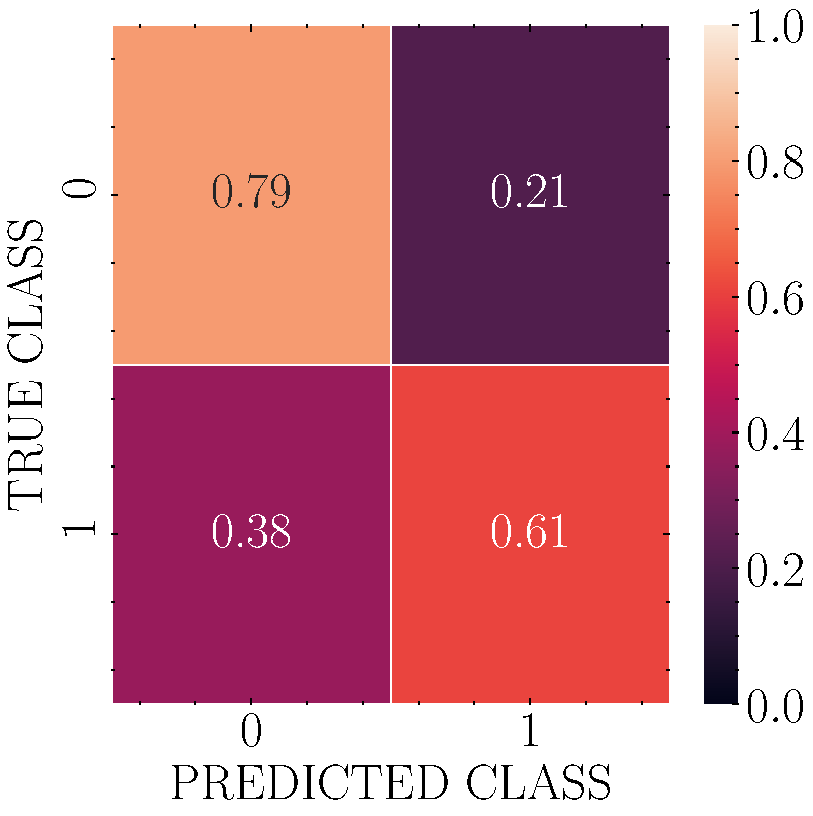
\includegraphics[width=1.5in]{../results/ex1/conf_mtx_QD_ML_dataset_P1a_size_10.pdf}
       \caption{QDA on P1a, size $10$.}
       \label{fig:QDA_P1a_10}
    \end{subfigure}
\quad
    \begin{subfigure}[!htbp]{0.24\textwidth}
       \centering
       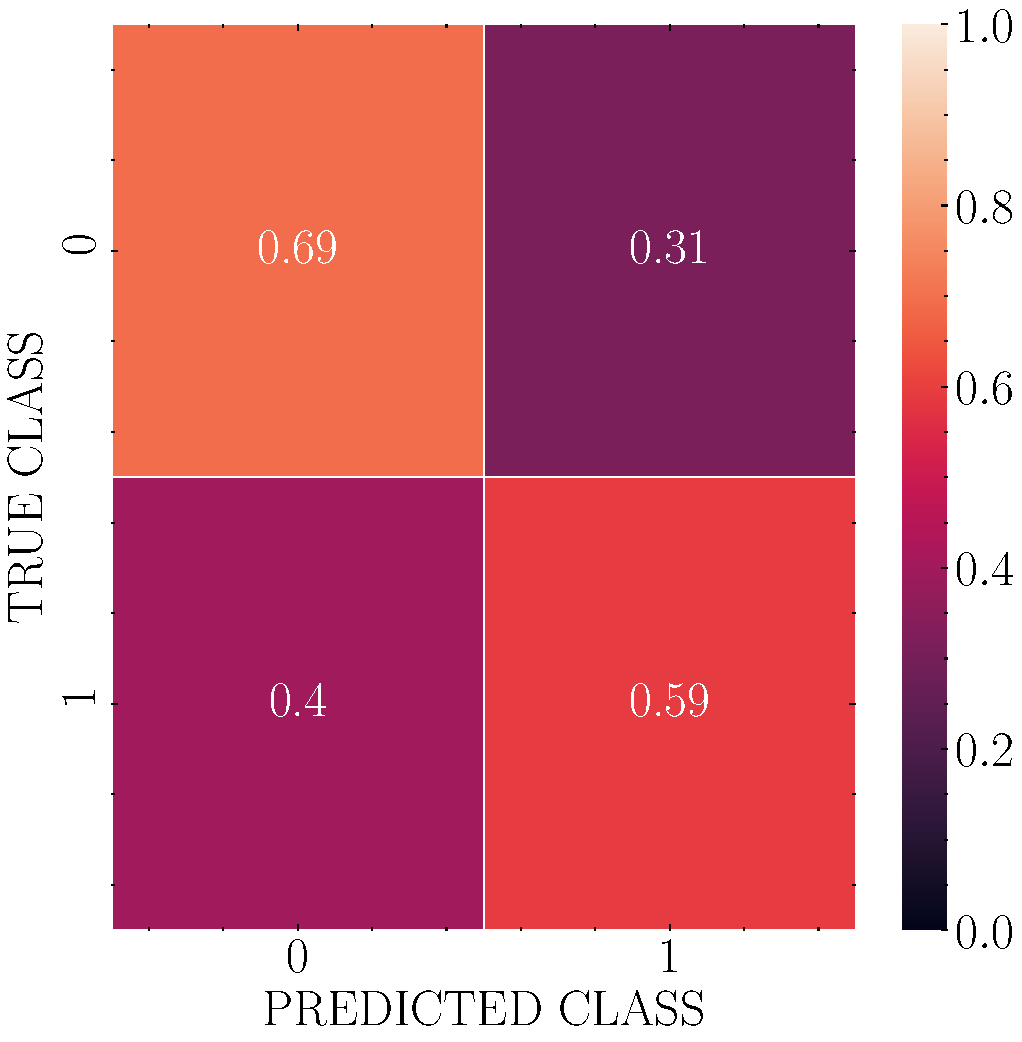
\includegraphics[width=1.5in]{../results/ex1/conf_mtx_KNN_dataset_P1a_size_10.pdf}
       \caption{KNN on P1a, size $10$.}
       \label{fig:KNN_P1a_10}
    \end{subfigure}
\quad
    \begin{subfigure}[!htbp]{0.24\textwidth}
       \centering
       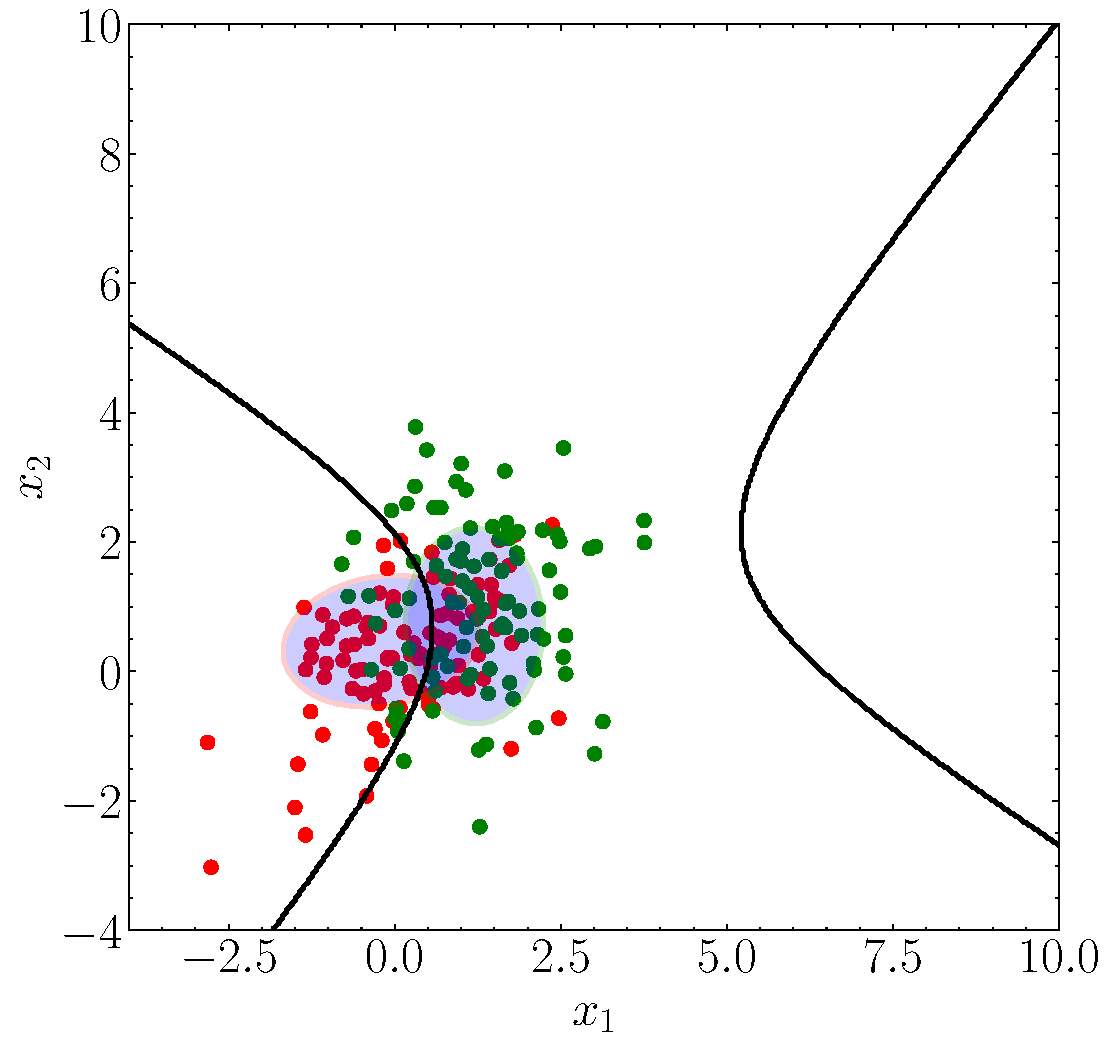
\includegraphics[width=1.5in]{../results/ex1/samples_QD_ML_dataset_P1a_size_10.pdf}
       \caption{Discriminant, size $10$.}
       \label{fig:DF_P1a_10}
    \end{subfigure}
    
\quad    
    \begin{subfigure}[!htbp]{0.24\textwidth}
       \centering
       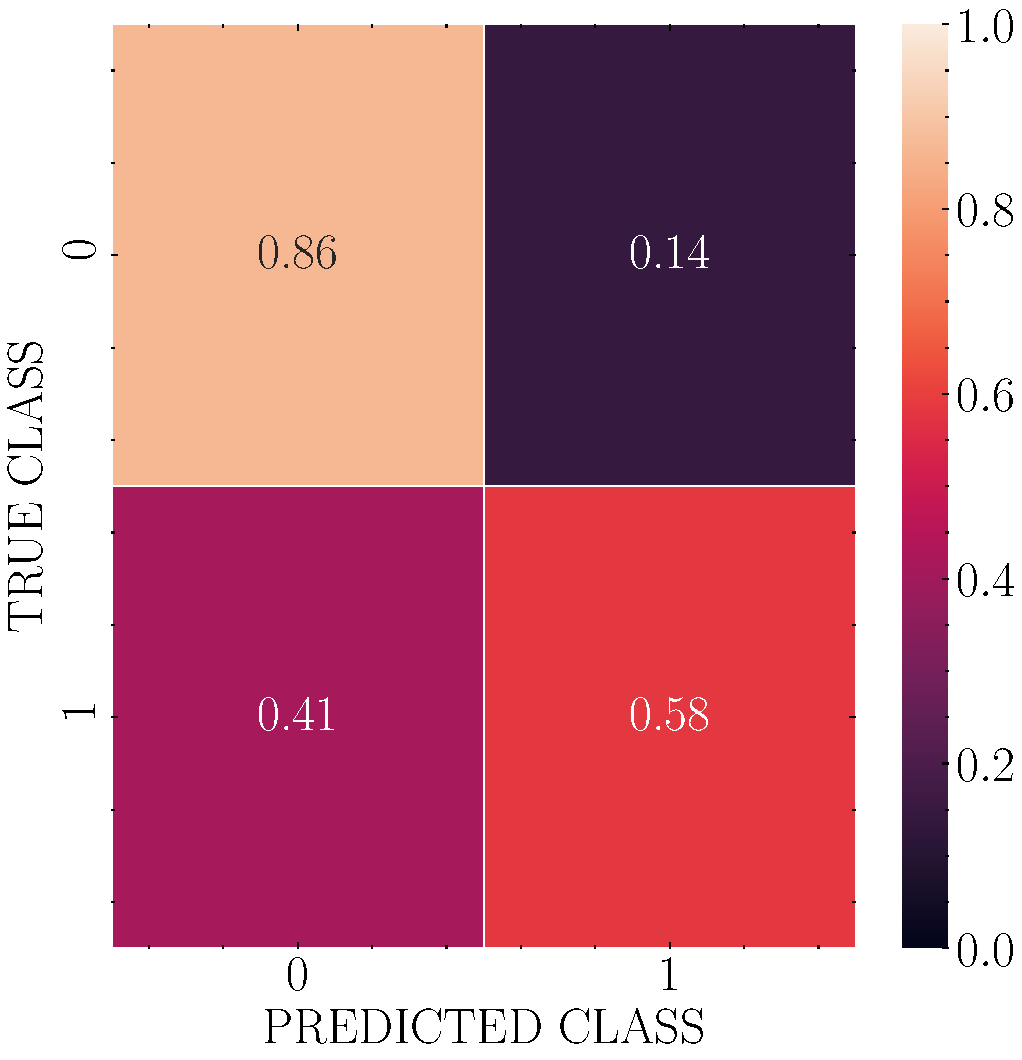
\includegraphics[width=1.5in]{../results/ex1/conf_mtx_QD_ML_dataset_P1a_size_25.pdf}
       \caption{QDA on P1a, size $25$.}
       \label{fig:QDA_P1a_25}
    \end{subfigure}
\quad    
    \begin{subfigure}[!htbp]{0.24\textwidth}
       \centering
       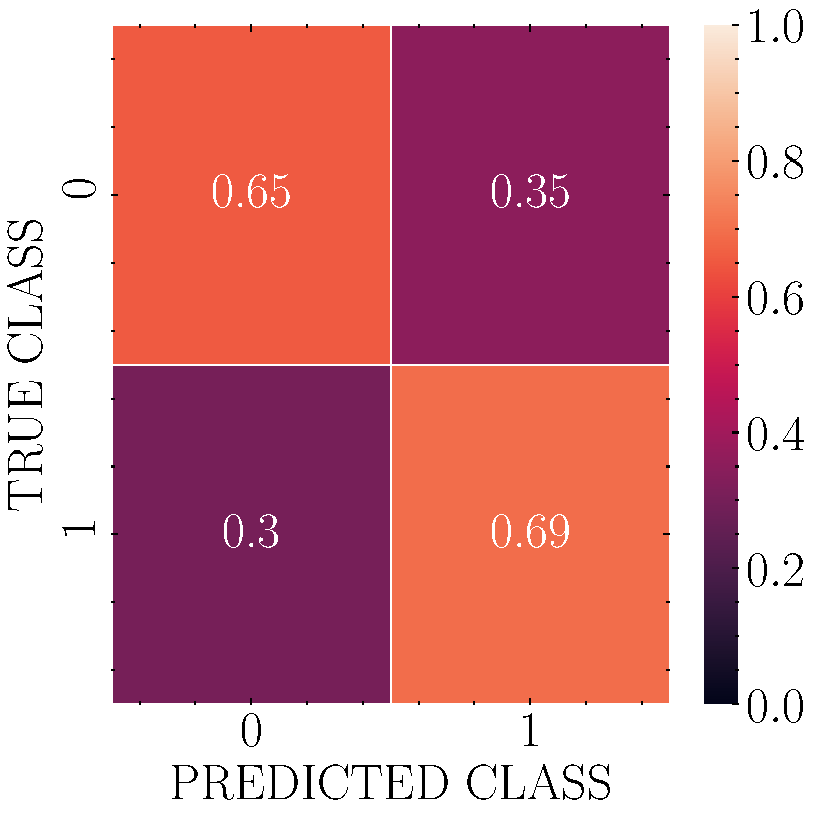
\includegraphics[width=1.5in]{../results/ex1/conf_mtx_KNN_dataset_P1a_size_25.pdf}
       \caption{KNN on P1a, size $25$.}
       \label{fig:KNN_P1a_25}
    \end{subfigure}
\quad
    \begin{subfigure}[!htbp]{0.24\textwidth}
       \centering
       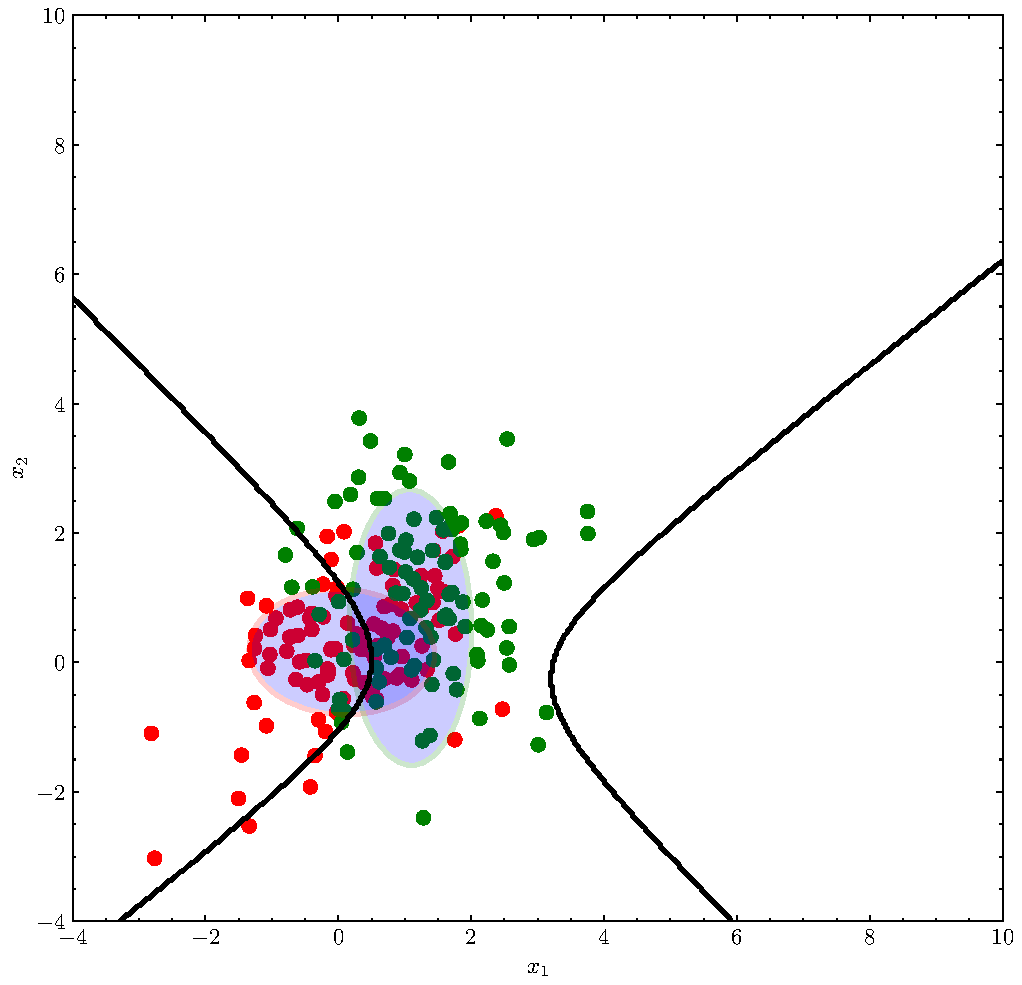
\includegraphics[width=1.5in]{../results/ex1/samples_QD_ML_dataset_P1a_size_25.pdf}
       \caption{Discriminant, size $25$.}
       \label{fig:DF_P1a_25}
    \end{subfigure}
    
\quad    
    \begin{subfigure}[!htbp]{0.24\textwidth}
       \centering
       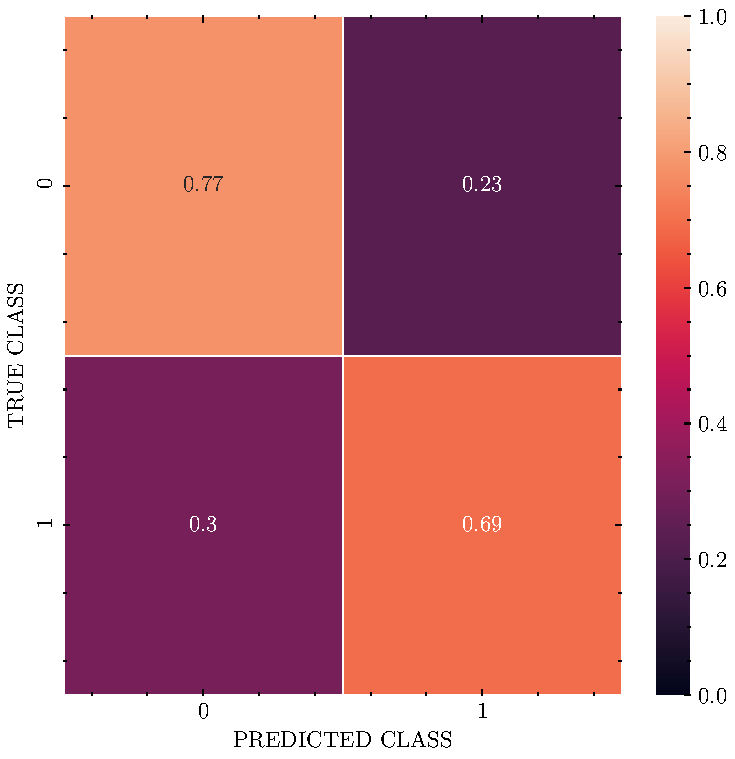
\includegraphics[width=1.5in]{../results/ex1/conf_mtx_QD_ML_dataset_P1a_size_75.pdf}
       \caption{QDA on P1a, size $75$.}
       \label{fig:QDA_P1a_75}
    \end{subfigure}
\quad    
    \begin{subfigure}[!htbp]{0.24\textwidth}
       \centering
       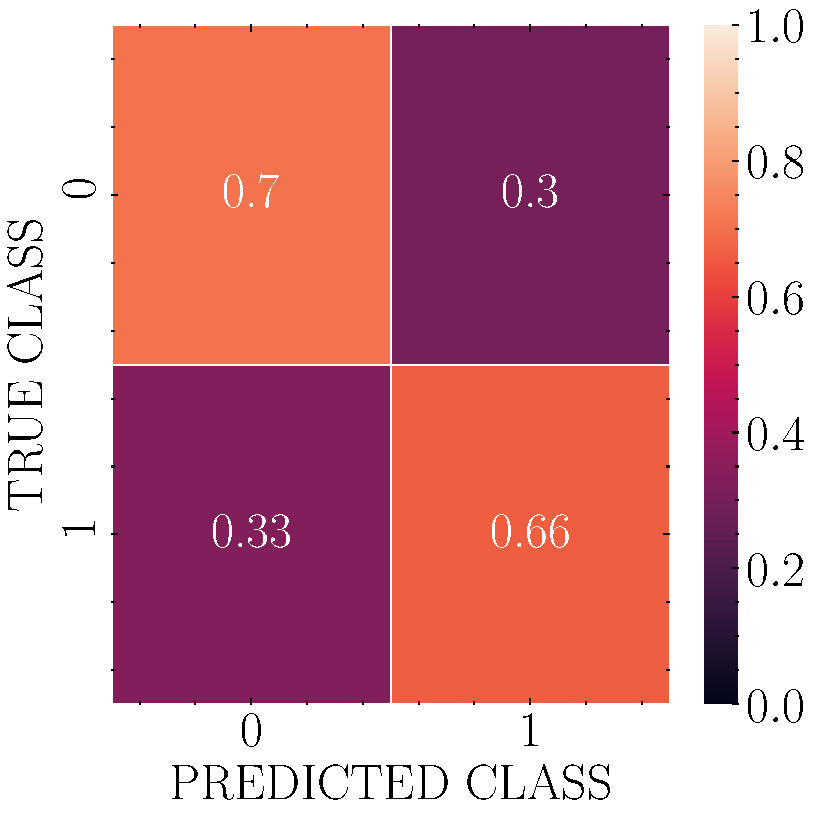
\includegraphics[width=1.5in]{../results/ex1/conf_mtx_KNN_dataset_P1a_size_75.pdf}
       \caption{KNN on P1a, size $75$.}
       \label{fig:KNN_P1a_75}
    \end{subfigure}
\quad
    \begin{subfigure}[!htbp]{0.24\textwidth}
       \centering
       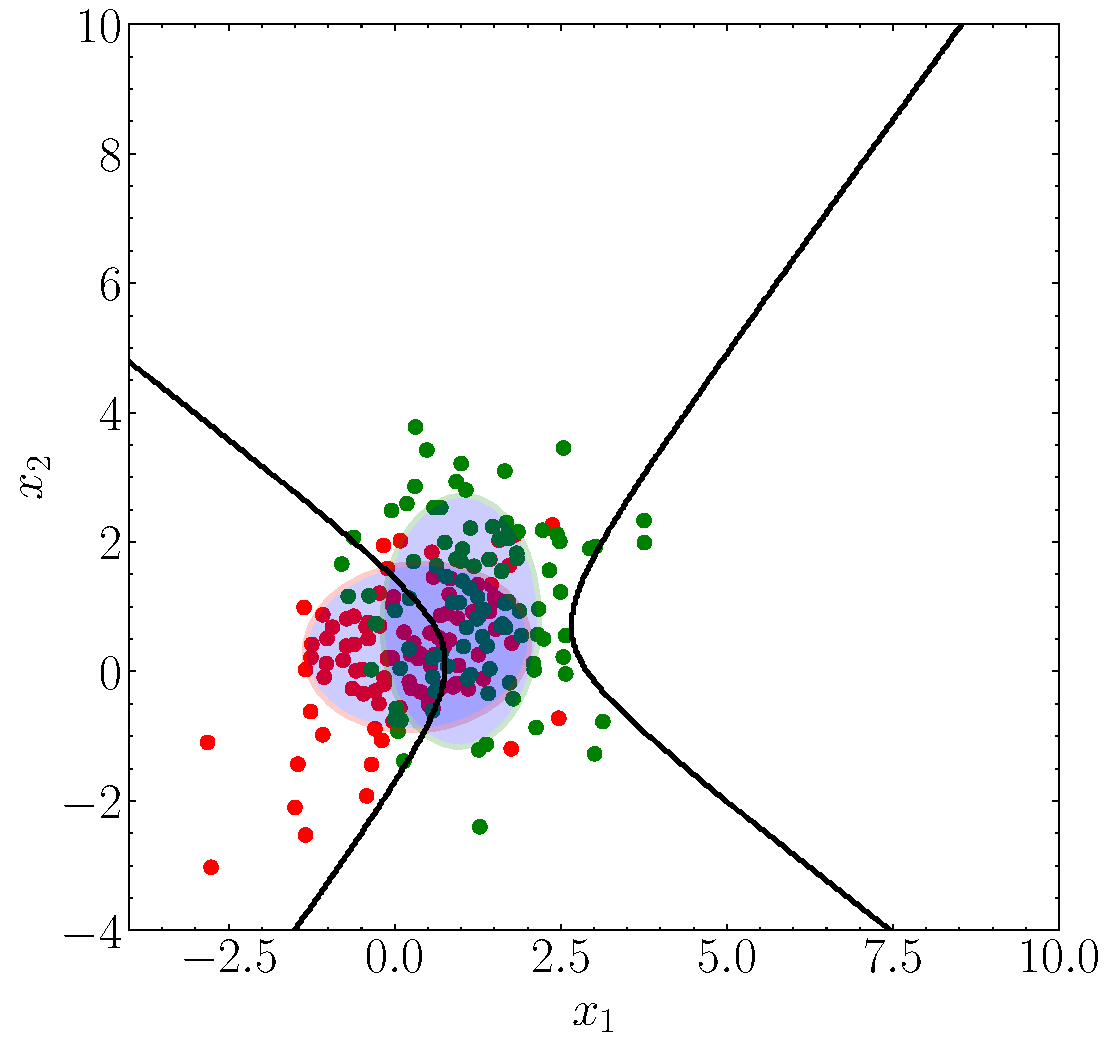
\includegraphics[width=1.5in]{../results/ex1/samples_QD_ML_dataset_P1a_size_75.pdf}
       \caption{Discriminant, size $75$.}
       \label{fig:DF_P1a_75}
    \end{subfigure}
    
\quad    
    \begin{subfigure}[!htbp]{0.24\textwidth}
       \centering
       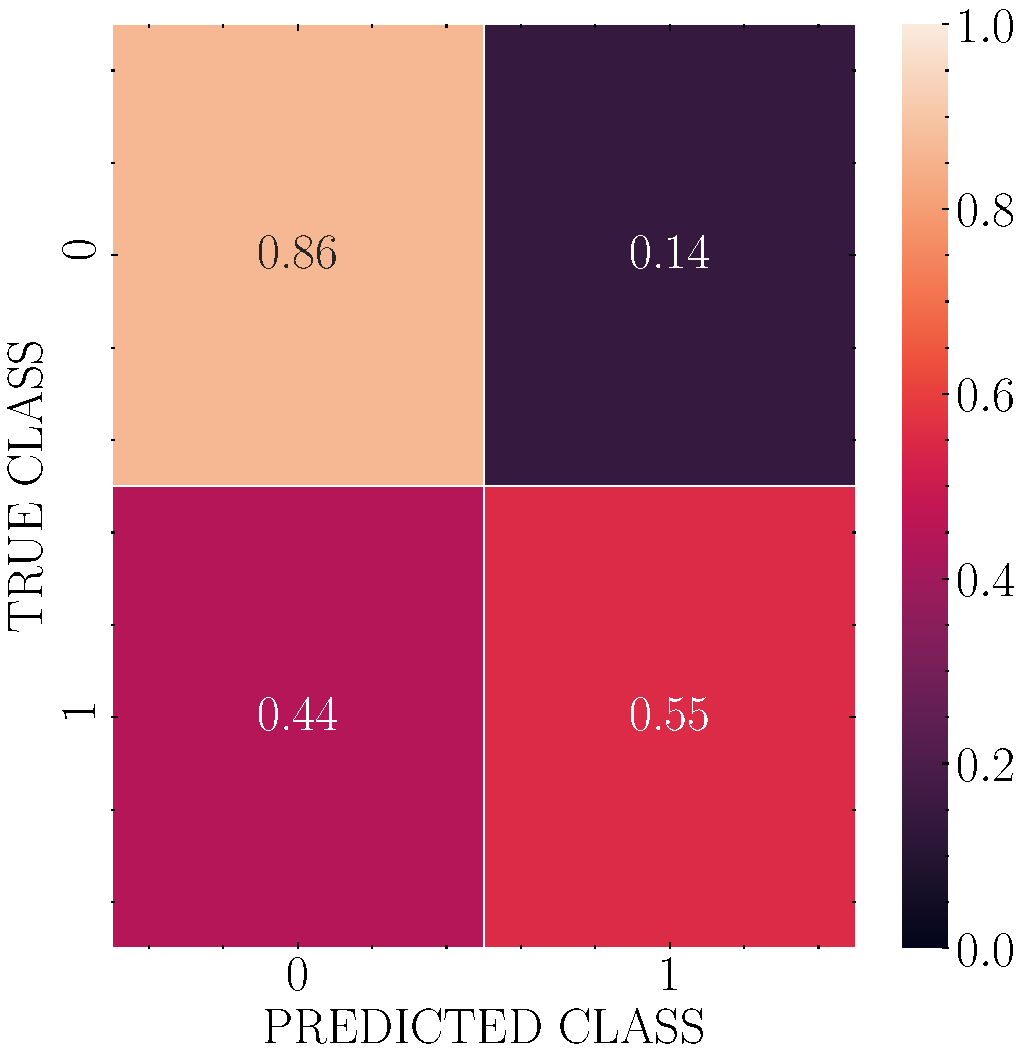
\includegraphics[width=1.5in]{../results/ex1/conf_mtx_QD_ML_dataset_P1a_size_199.pdf}
       \caption{QDA on P1a, size $199$.}
       \label{fig:QDA_P1a_199}
    \end{subfigure}
\quad    
    \begin{subfigure}[!htbp]{0.24\textwidth}
       \centering
       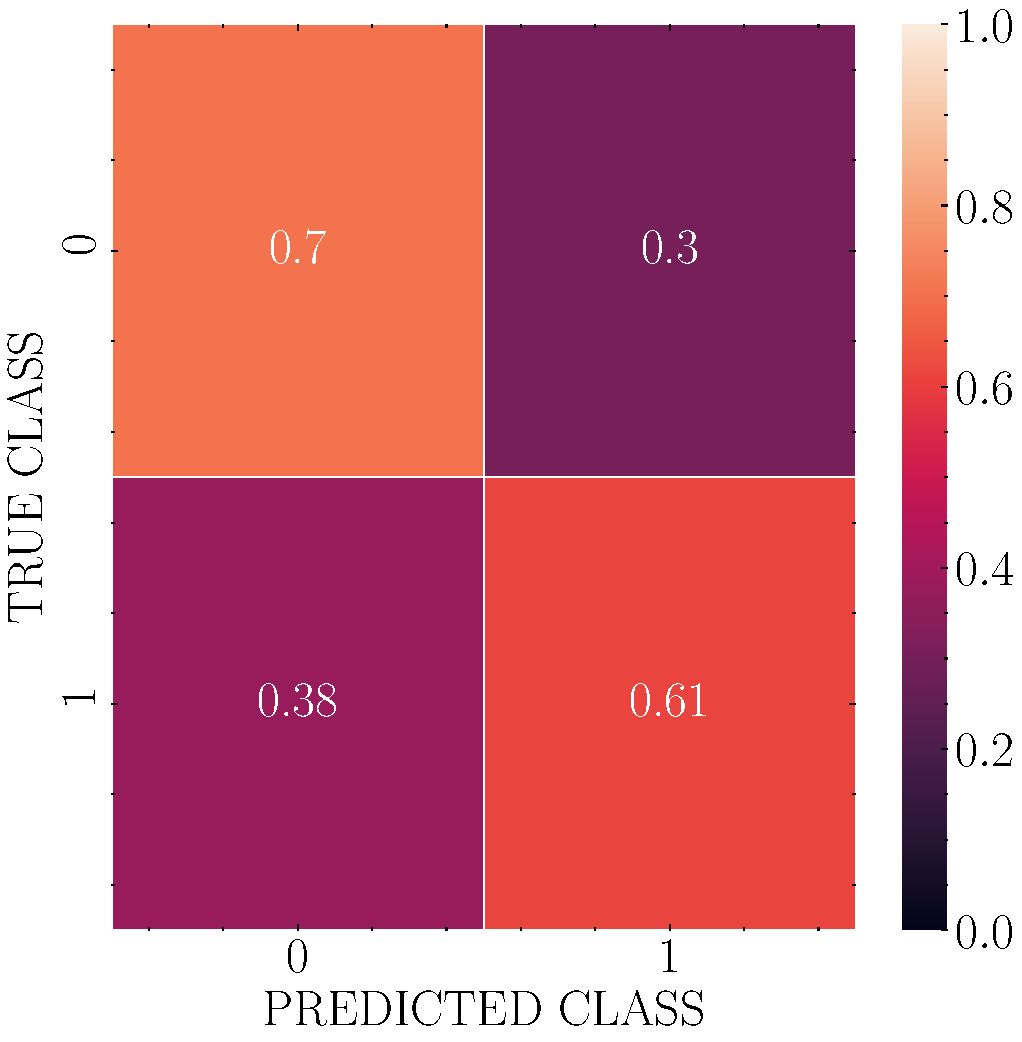
\includegraphics[width=1.5in]{../results/ex1/conf_mtx_KNN_dataset_P1a_size_199.pdf}
       \caption{KNN on P1a, size $199$.}
       \label{fig:KNN_P1a_199}
    \end{subfigure}
\quad
    \begin{subfigure}[!htbp]{0.24\textwidth}
       \centering
       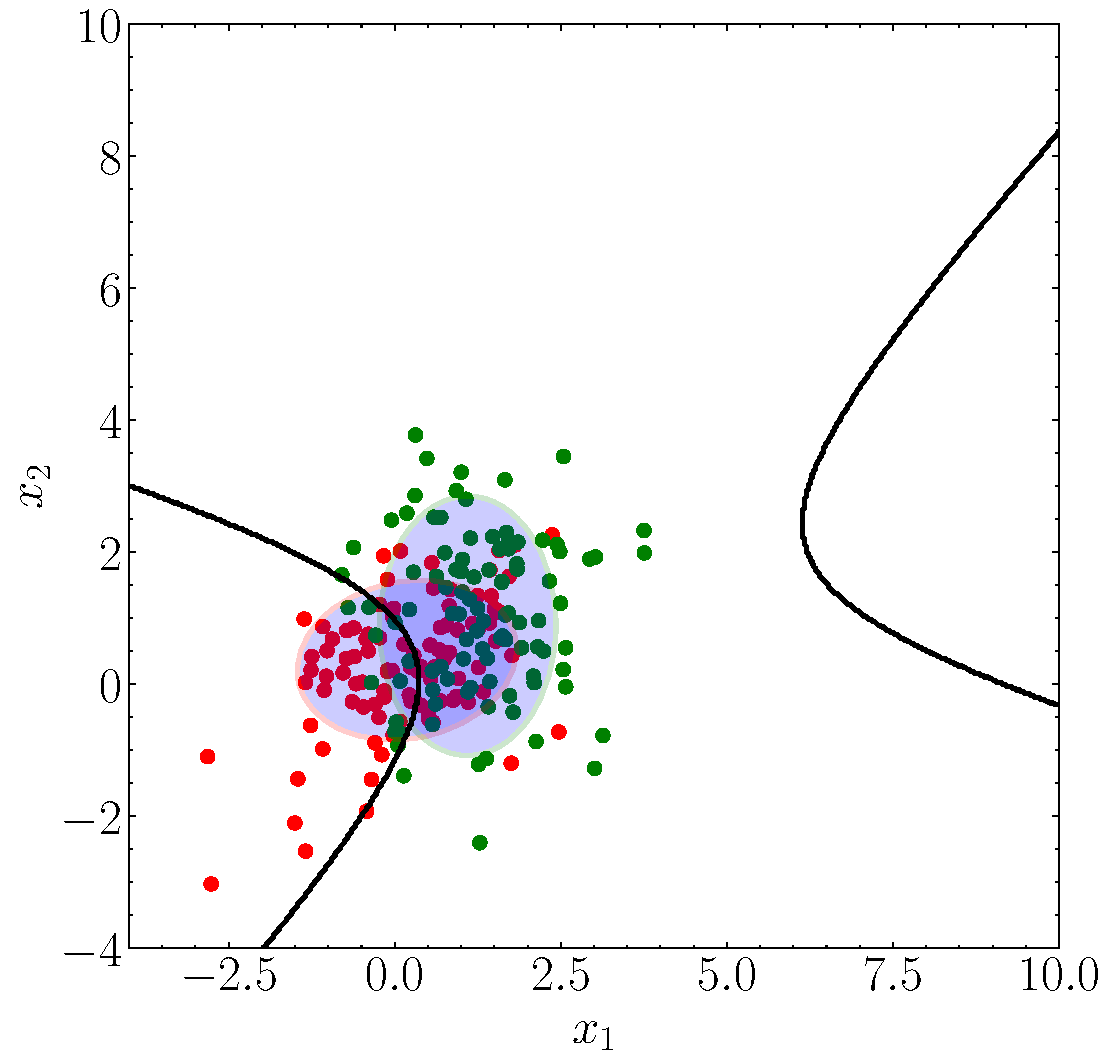
\includegraphics[width=1.5in]{../results/ex1/samples_QD_ML_dataset_P1a_size_199.pdf}
       \caption{Discriminant, size $199$.}
       \label{fig:DF_P1a_199}
    \end{subfigure}

\caption{Bayes classifier and Nearest neighbour classification on P1a dataset.}
\label{fig:ex11P1a}
\end{figure}

{\it Inferences on P1b}: The class means are $\bmu_{0} = [0,0]^{\TT}$ and $\bmu_{1} = [3,3]^{\TT}$, and the covariances are in the same order. The class distributions are farther apart, i.e., the discriminability is higher than in P1a. This is seen with the training samples from each class barely overlapping into the other class. Within this setting, the classifiers trained with training sizes $10$, $25$, $75$, and $199$ on the average show, show an increasing trend in test accuracy. The nearest-neighbour classifier performs comparably to the Bayes' classifier. In no case, the error in classification using nearest-neighbour classifier exceeds twice the error in the Bayes' classifier. With increasing size of the training set, the learnt Gaussians is observed to learn ``better'', i.e., the means and covariances are closer to the true values.

\begin{figure}[!htbp]
\centering
    \begin{subfigure}[!htbp]{0.24\textwidth}
       \centering
       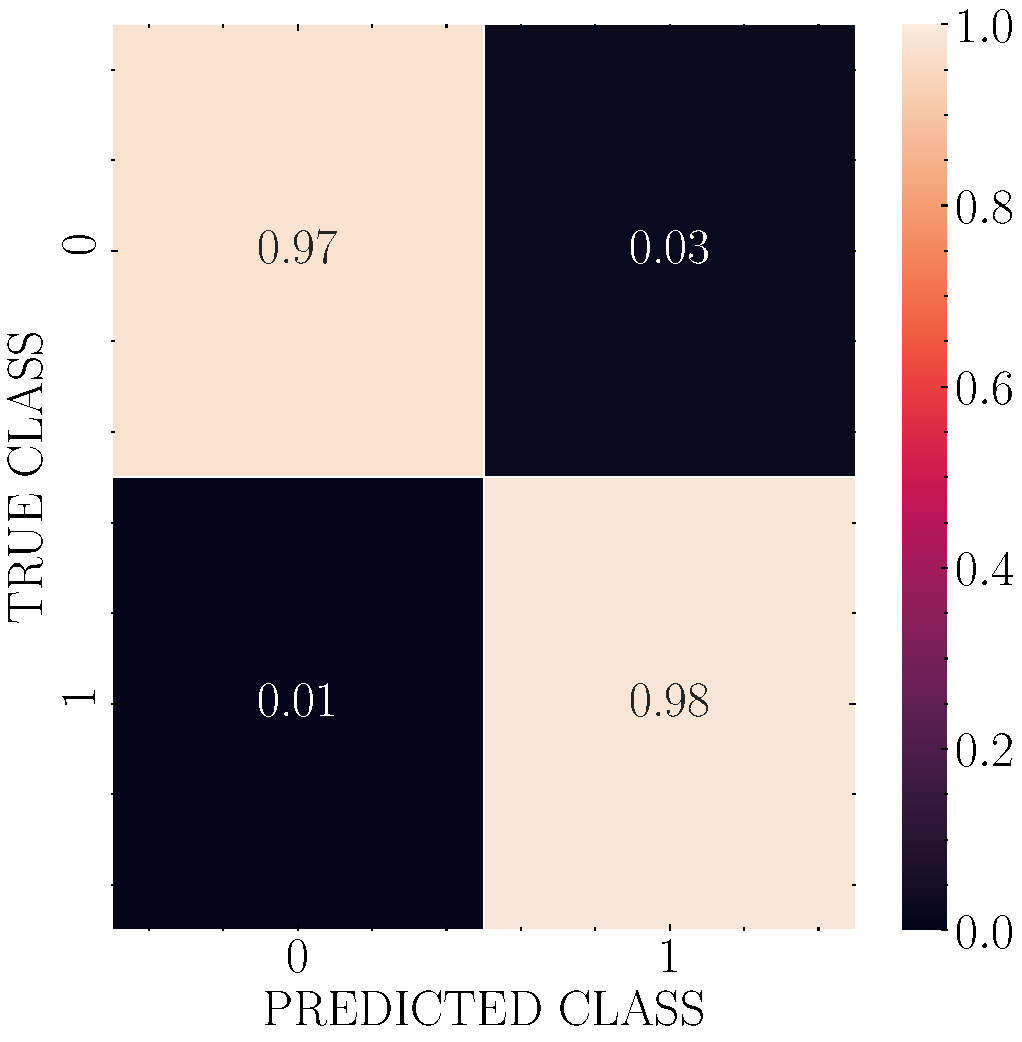
\includegraphics[width=1.5in]{../results/ex1/conf_mtx_QD_ML_dataset_P1b_size_10.pdf}
       \caption{QDA on P1b, size $10$.}
       \label{fig:QDA_P1b_10}
    \end{subfigure}
\quad
    \begin{subfigure}[!htbp]{0.24\textwidth}
       \centering
       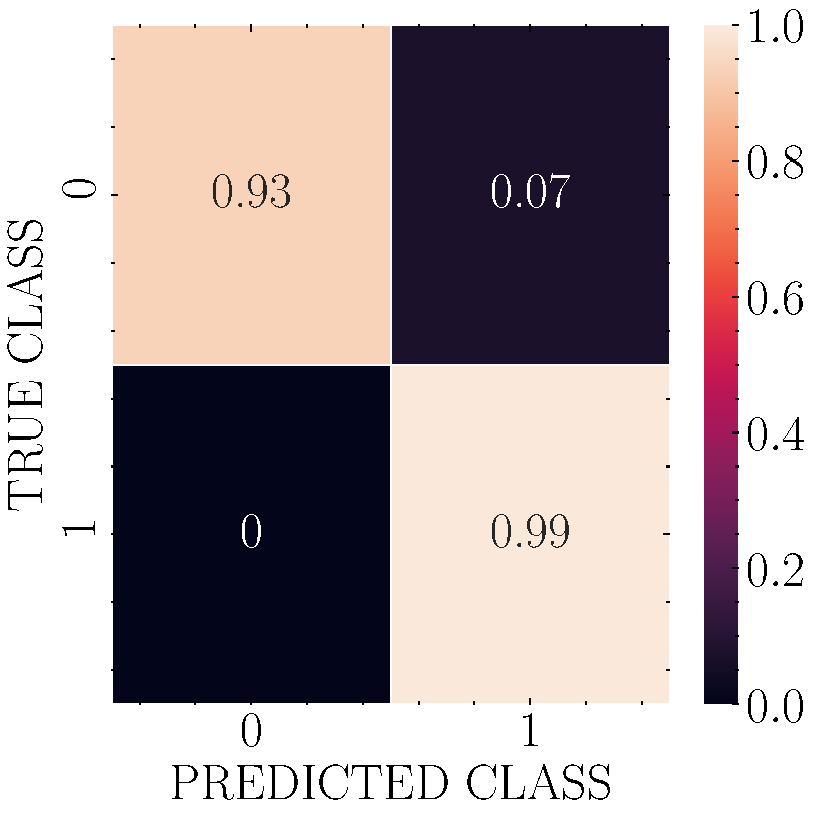
\includegraphics[width=1.5in]{../results/ex1/conf_mtx_KNN_dataset_P1b_size_10.pdf}
       \caption{KNN on P1b, size $10$.}
       \label{fig:KNN_P1b_10}
    \end{subfigure}
\quad
    \begin{subfigure}[!htbp]{0.24\textwidth}
       \centering
       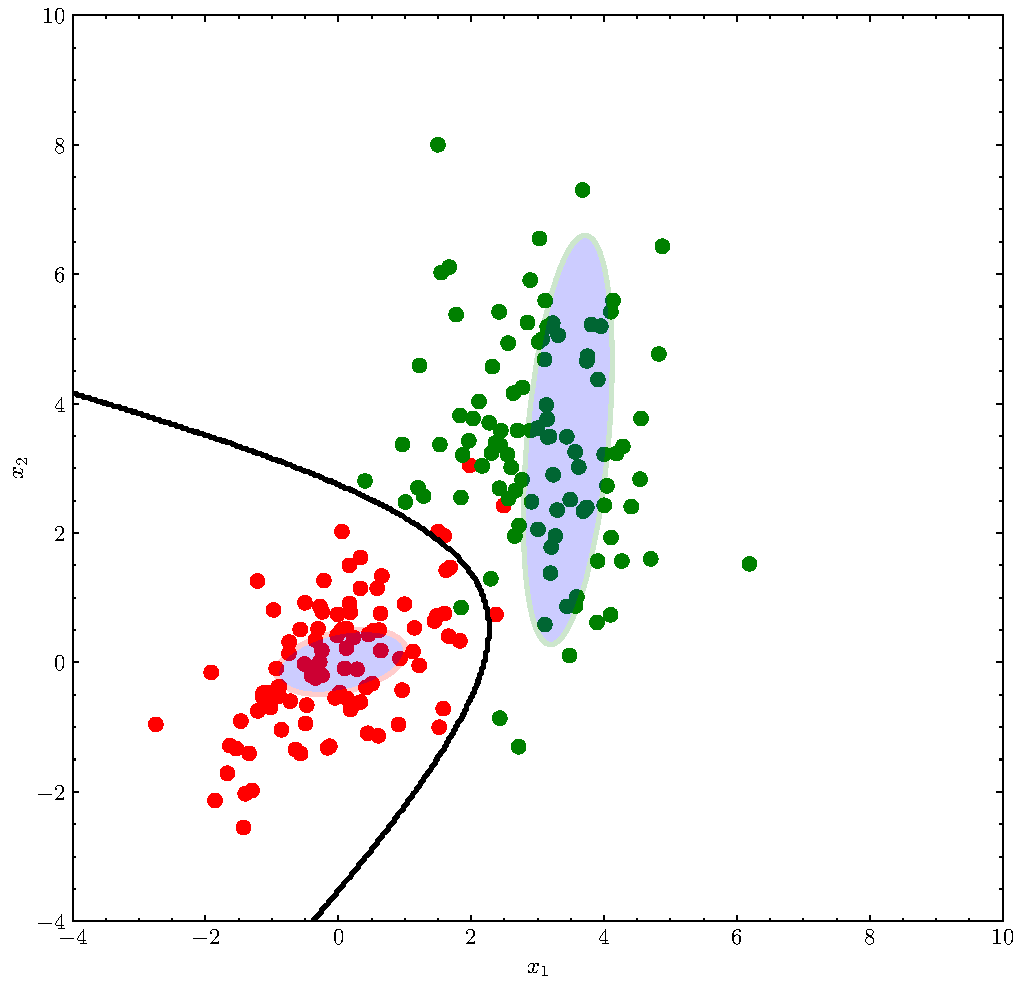
\includegraphics[width=1.5in]{../results/ex1/samples_QD_ML_dataset_P1b_size_10.pdf}
       \caption{Discriminant, size $10$.}
       \label{fig:KNN_P1b_10}
    \end{subfigure}
    
\quad    
    \begin{subfigure}[!htbp]{0.24\textwidth}
       \centering
       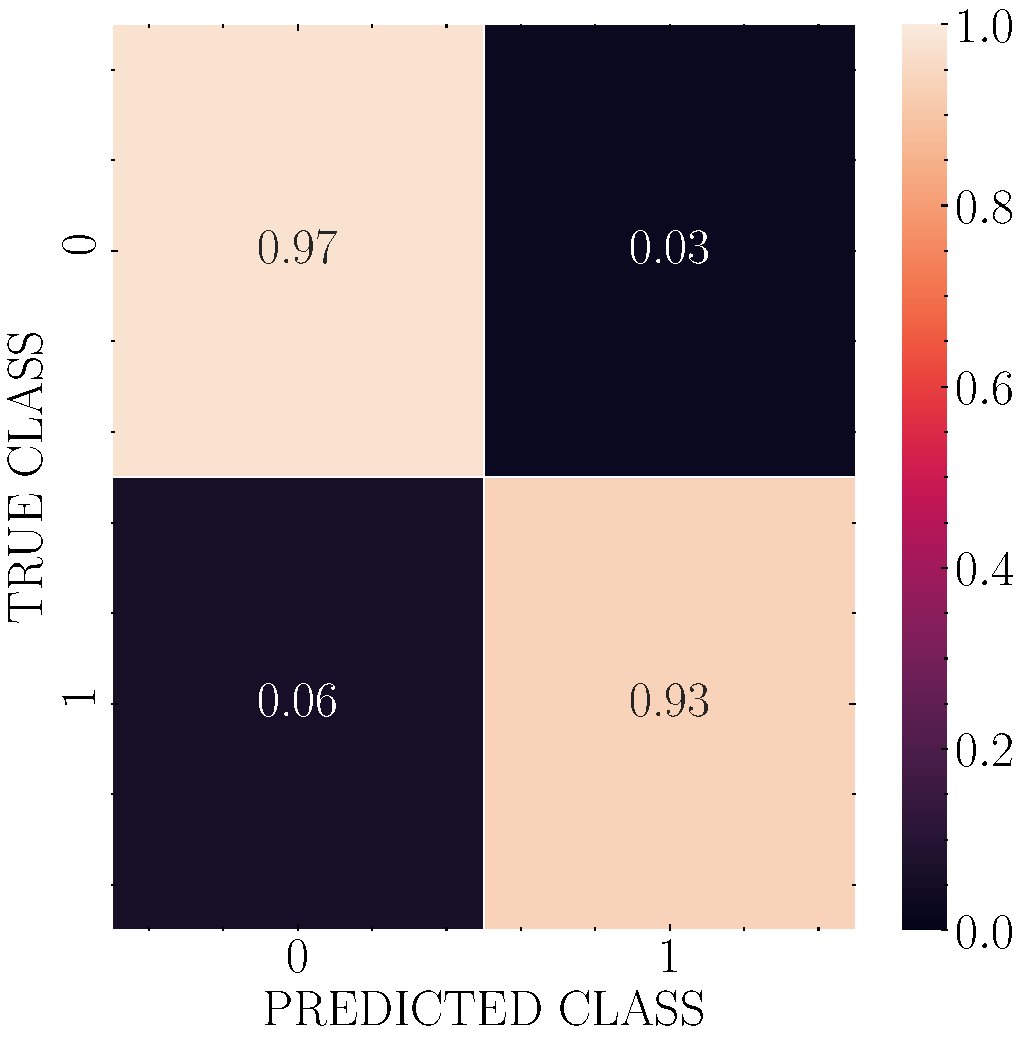
\includegraphics[width=1.5in]{../results/ex1/conf_mtx_QD_ML_dataset_P1b_size_25.pdf}
       \caption{QDA on P1b, size $25$.}
       \label{fig:KNN_P1b_25}
    \end{subfigure}
\quad    
    \begin{subfigure}[!htbp]{0.24\textwidth}
       \centering
       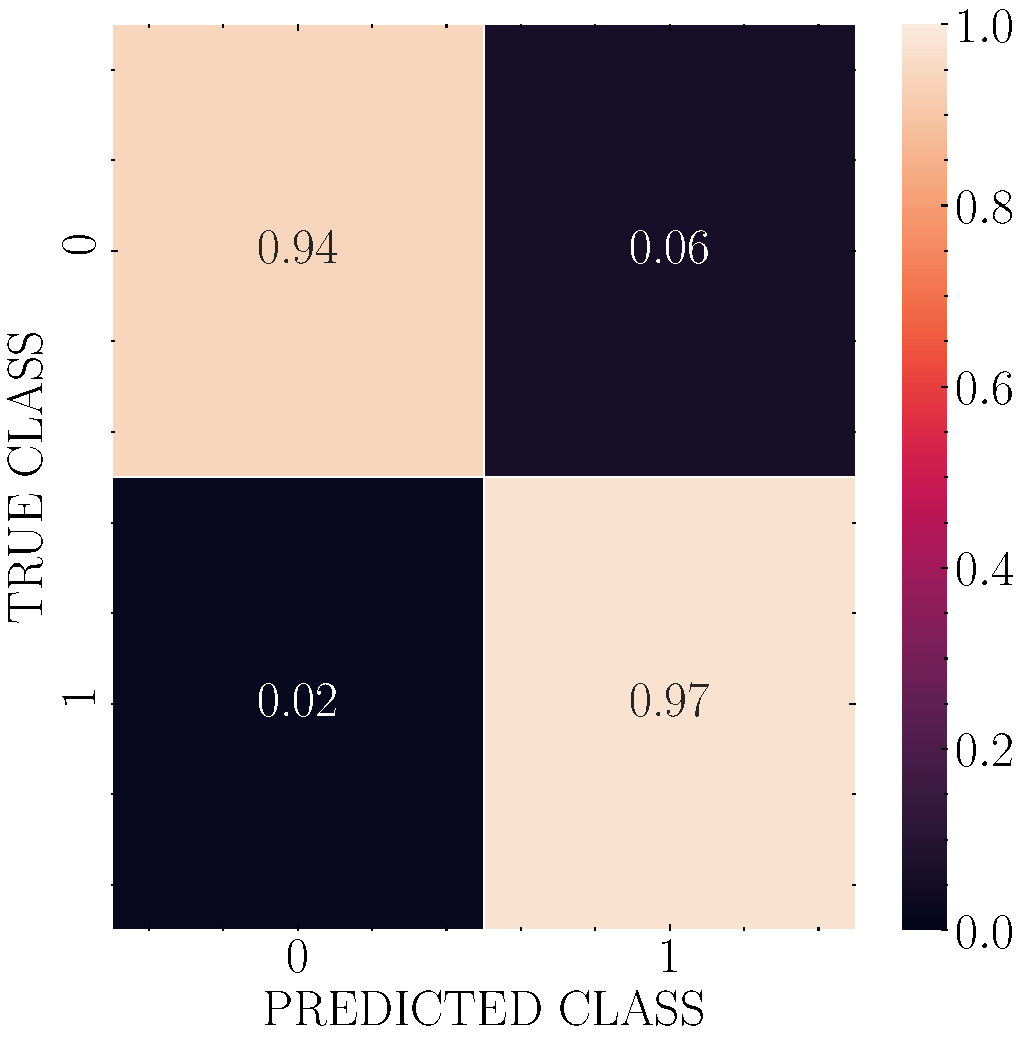
\includegraphics[width=1.5in]{../results/ex1/conf_mtx_KNN_dataset_P1b_size_25.pdf}
       \caption{KNN on P1b, size $25$.}
       \label{fig:KNN_P1b_25}
    \end{subfigure}
\quad
    \begin{subfigure}[!htbp]{0.24\textwidth}
       \centering
       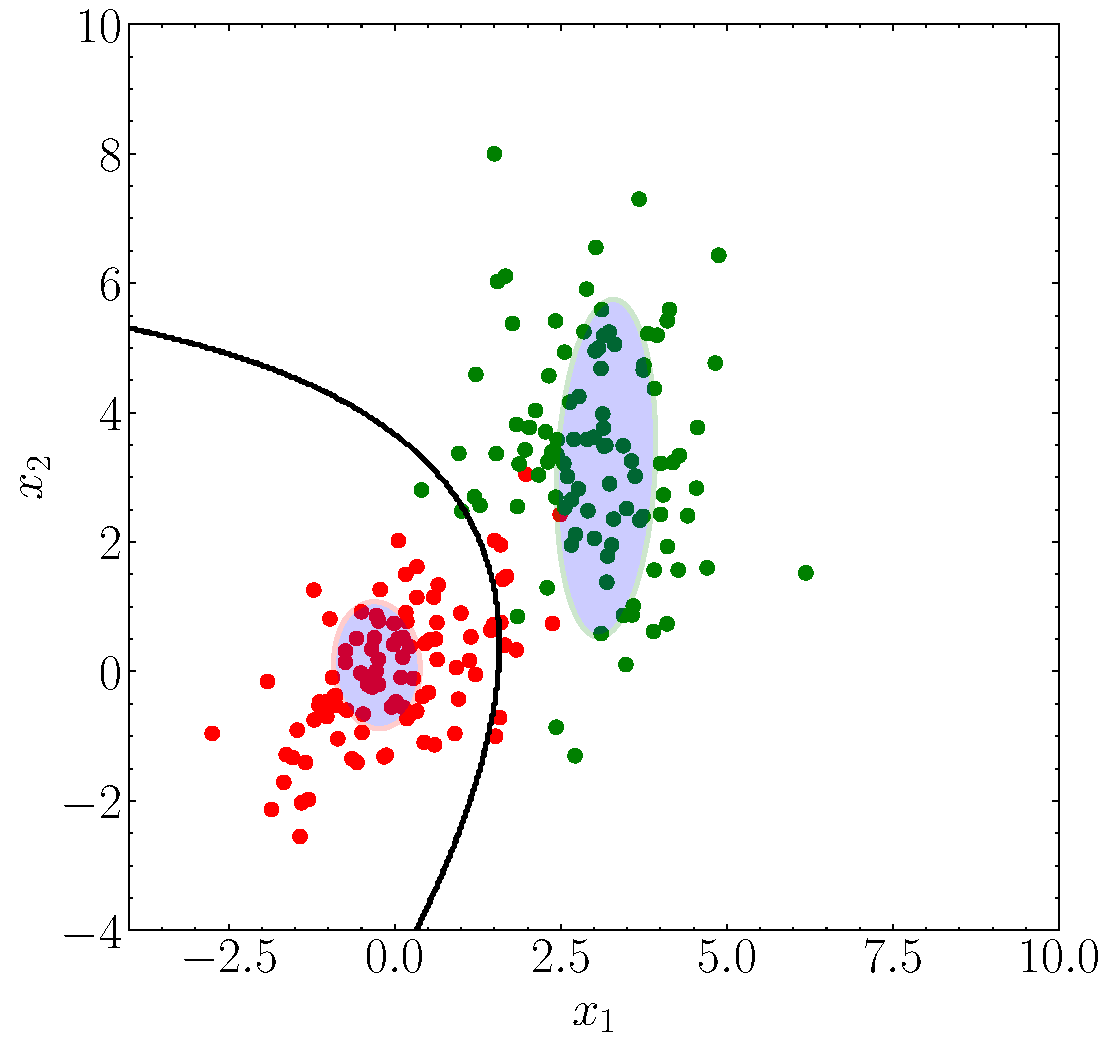
\includegraphics[width=1.5in]{../results/ex1/samples_QD_ML_dataset_P1b_size_25.pdf}
       \caption{Discriminant, size $25$.}
       \label{fig:KNN_P1b_25}
    \end{subfigure}
    
\quad    
    \begin{subfigure}[!htbp]{0.24\textwidth}
       \centering
       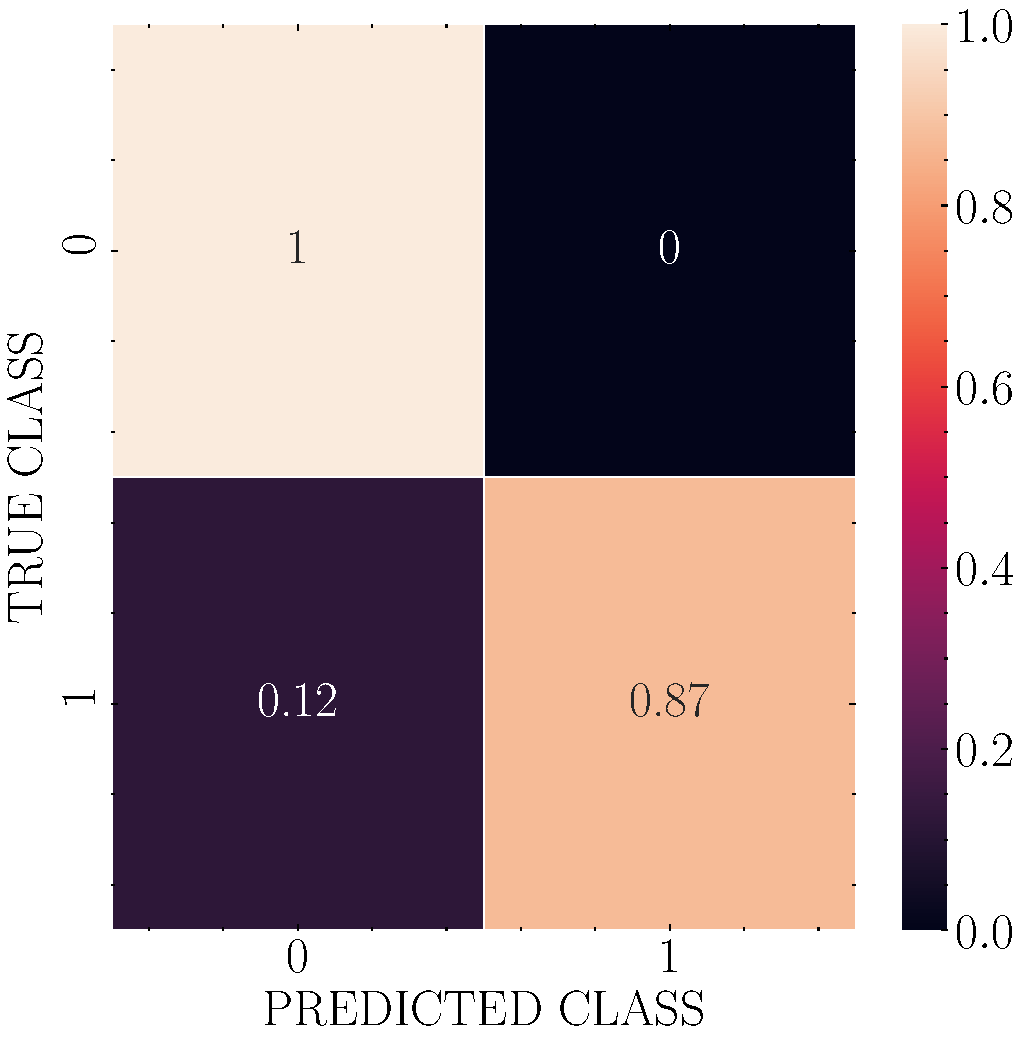
\includegraphics[width=1.5in]{../results/ex1/conf_mtx_QD_ML_dataset_P1b_size_75.pdf}
       \caption{QDA on P1b, size $75$.}
       \label{fig:KNN_P1b_75}
    \end{subfigure}
\quad    
    \begin{subfigure}[!htbp]{0.24\textwidth}
       \centering
       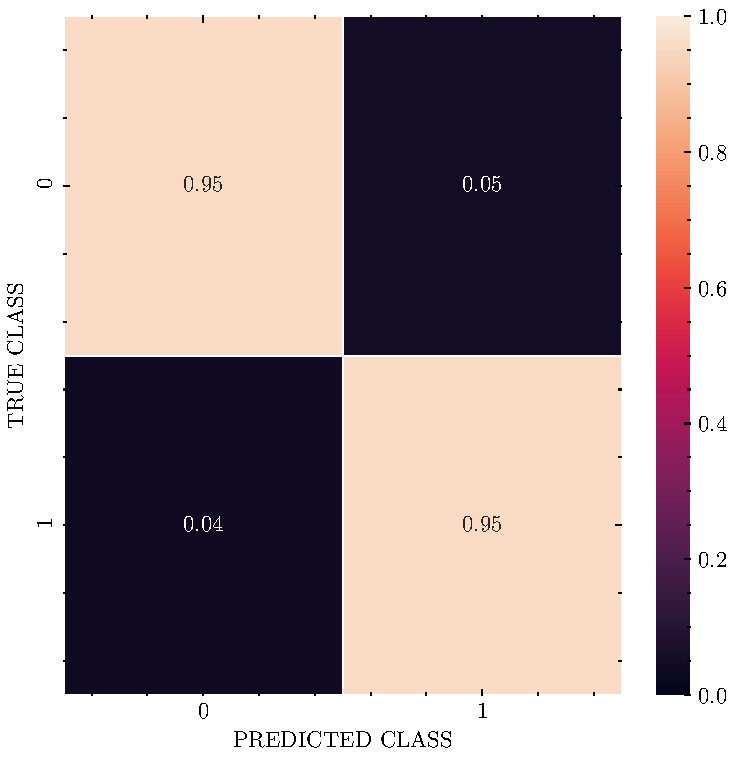
\includegraphics[width=1.5in]{../results/ex1/conf_mtx_KNN_dataset_P1b_size_75.pdf}
       \caption{KNN on P1b, size $75$.}
       \label{fig:KNN_P1b_75}
    \end{subfigure}
\quad
    \begin{subfigure}[!htbp]{0.24\textwidth}
       \centering
       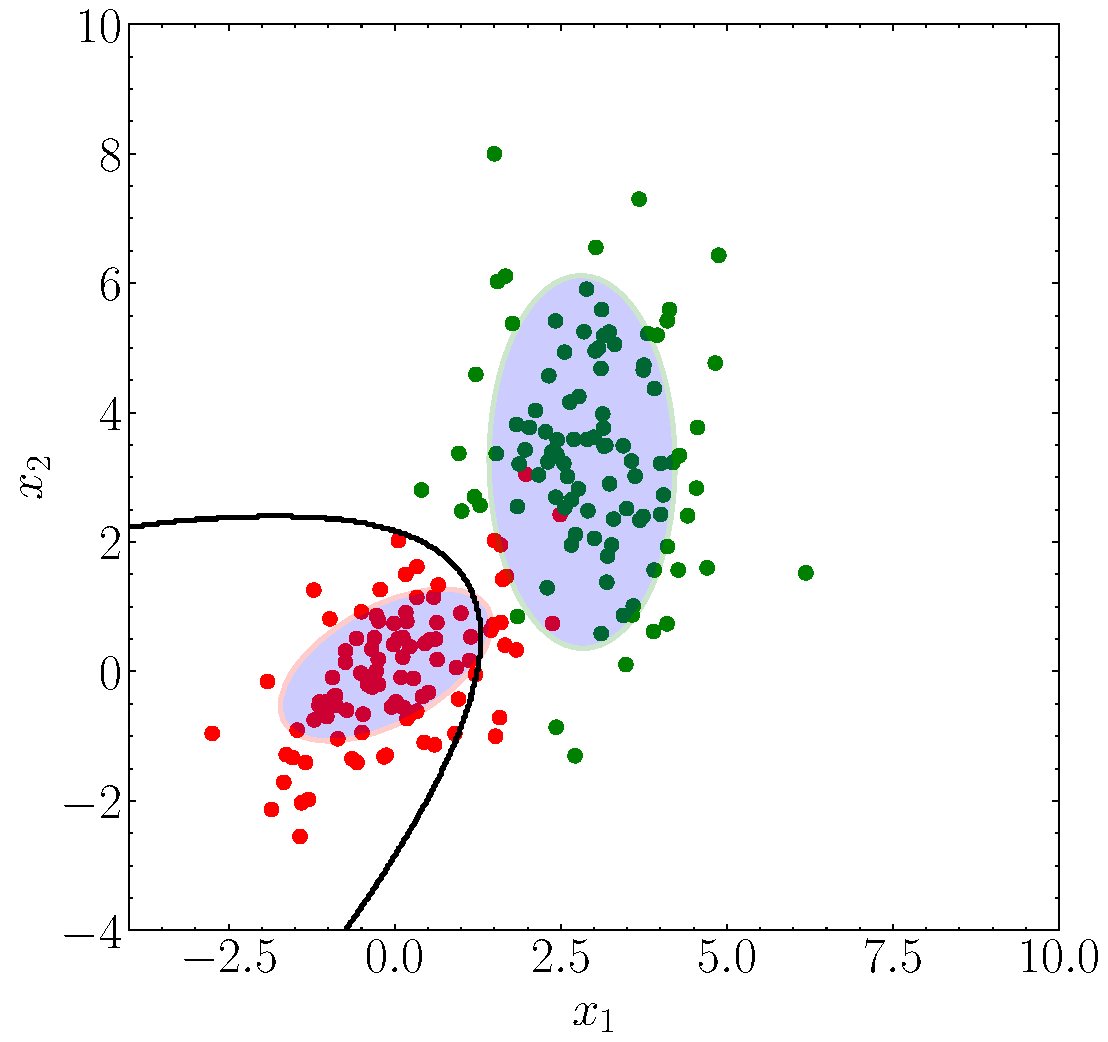
\includegraphics[width=1.5in]{../results/ex1/samples_QD_ML_dataset_P1b_size_75.pdf}
       \caption{Discriminant, size $75$.}
       \label{fig:KNN_P1b_75}
    \end{subfigure}
    
\quad    
    \begin{subfigure}[!htbp]{0.24\textwidth}
       \centering
       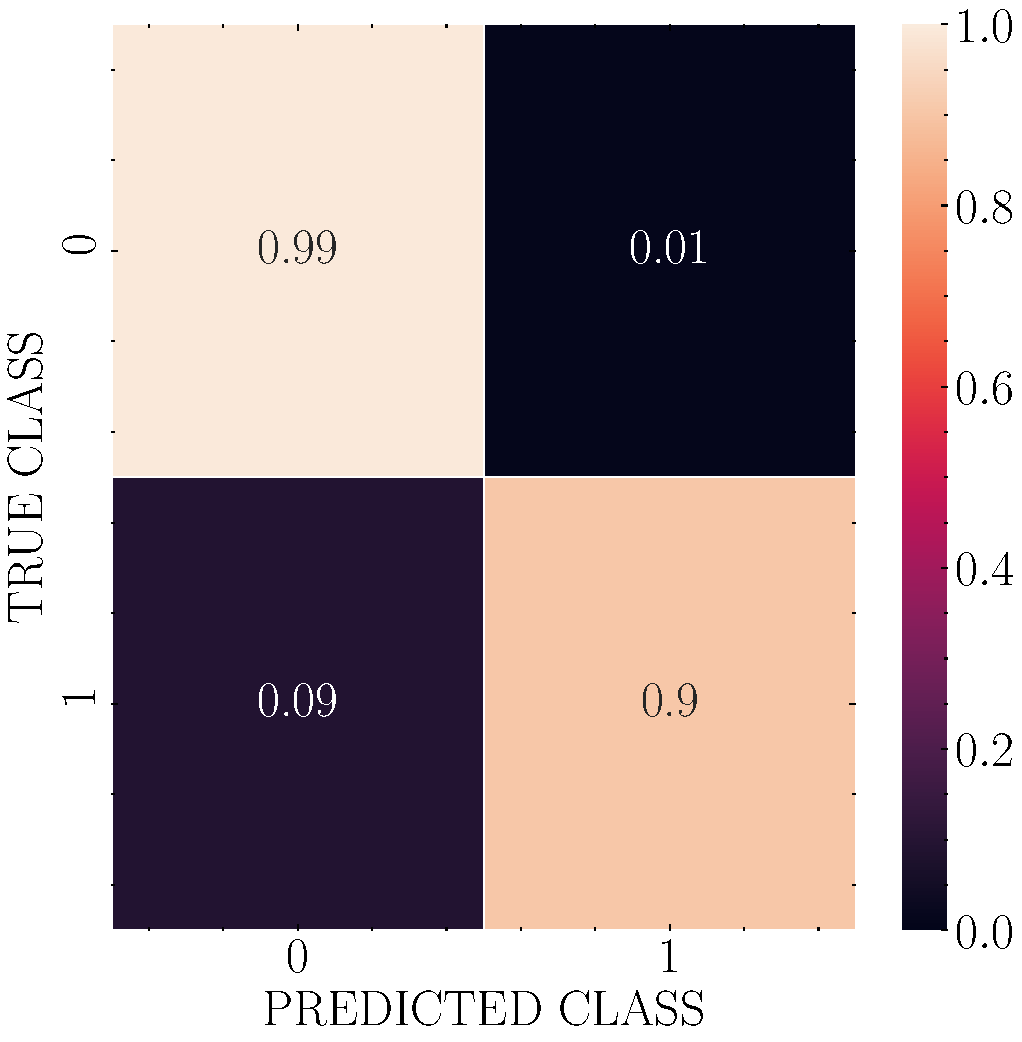
\includegraphics[width=1.5in]{../results/ex1/conf_mtx_QD_ML_dataset_P1b_size_199.pdf}
       \caption{QDA on P1b, size $199$.}
       \label{fig:KNN_P1b_199}
    \end{subfigure}
\quad    
    \begin{subfigure}[!htbp]{0.24\textwidth}
       \centering
       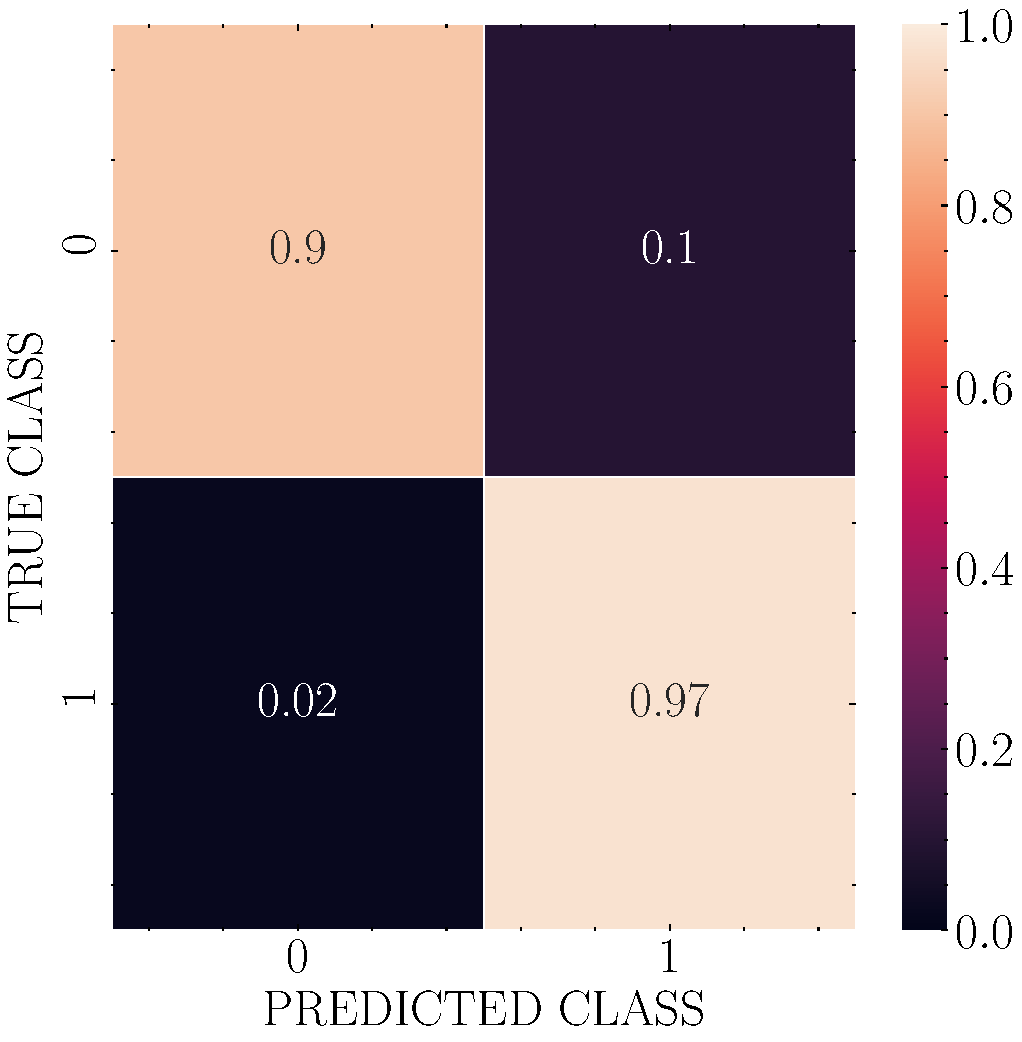
\includegraphics[width=1.5in]{../results/ex1/conf_mtx_KNN_dataset_P1b_size_199.pdf}
       \caption{KNN on P1b, size $199$.}
       \label{fig:KNN_P1b_199}
    \end{subfigure}
\quad
    \begin{subfigure}[!htbp]{0.24\textwidth}
       \centering
       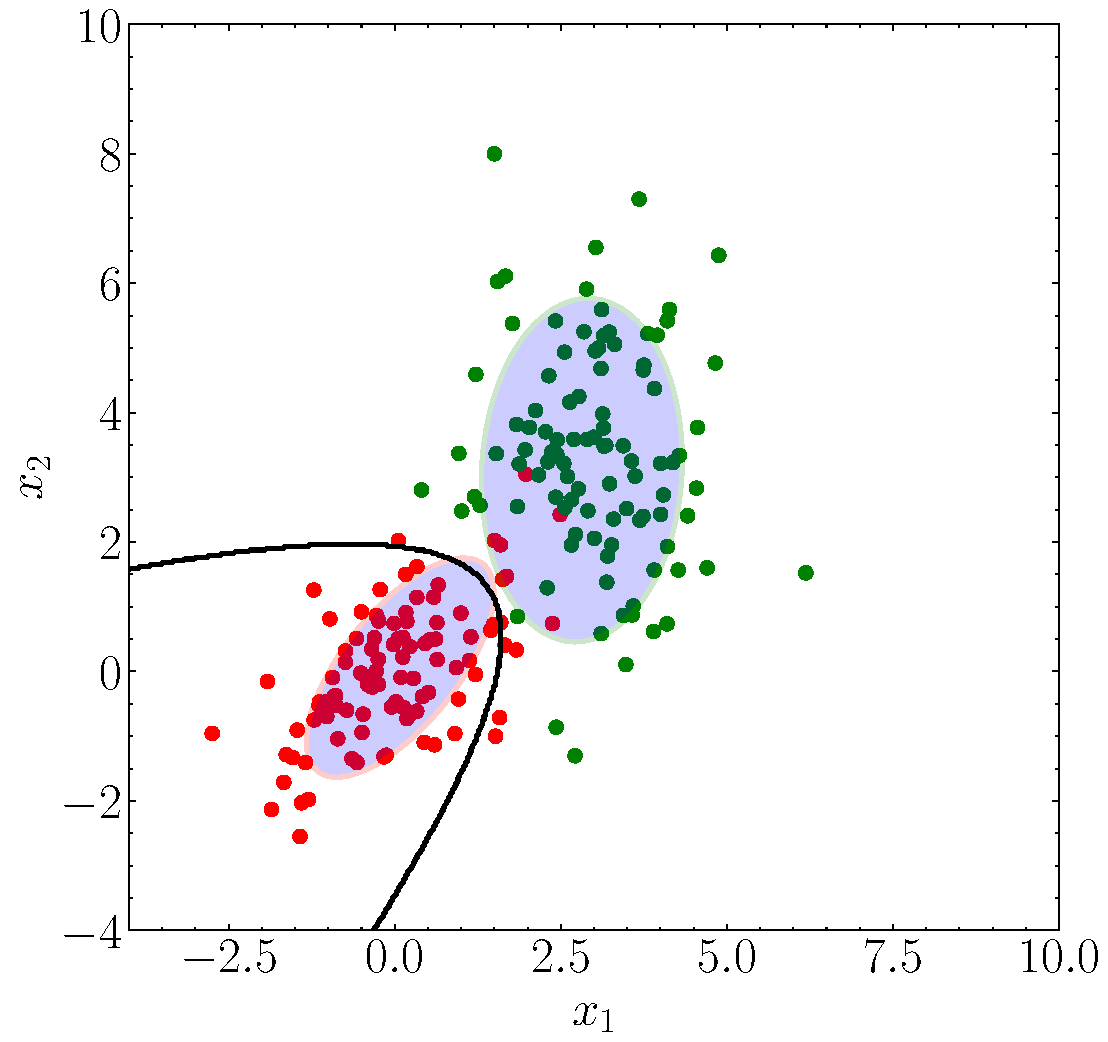
\includegraphics[width=1.5in]{../results/ex1/samples_QD_ML_dataset_P1b_size_199.pdf}
       \caption{Discriminant, size $199$.}
       \label{fig:KNN_P1b_199}
    \end{subfigure}

\caption{Bayes classifier and Nearest neighbour classification on P1b dataset.}
\label{fig:ex11P1b}
\end{figure}

\begin{figure}[!htbp]
\centering
    \begin{subfigure}[!htbp]{0.24\textwidth}
       \centering
       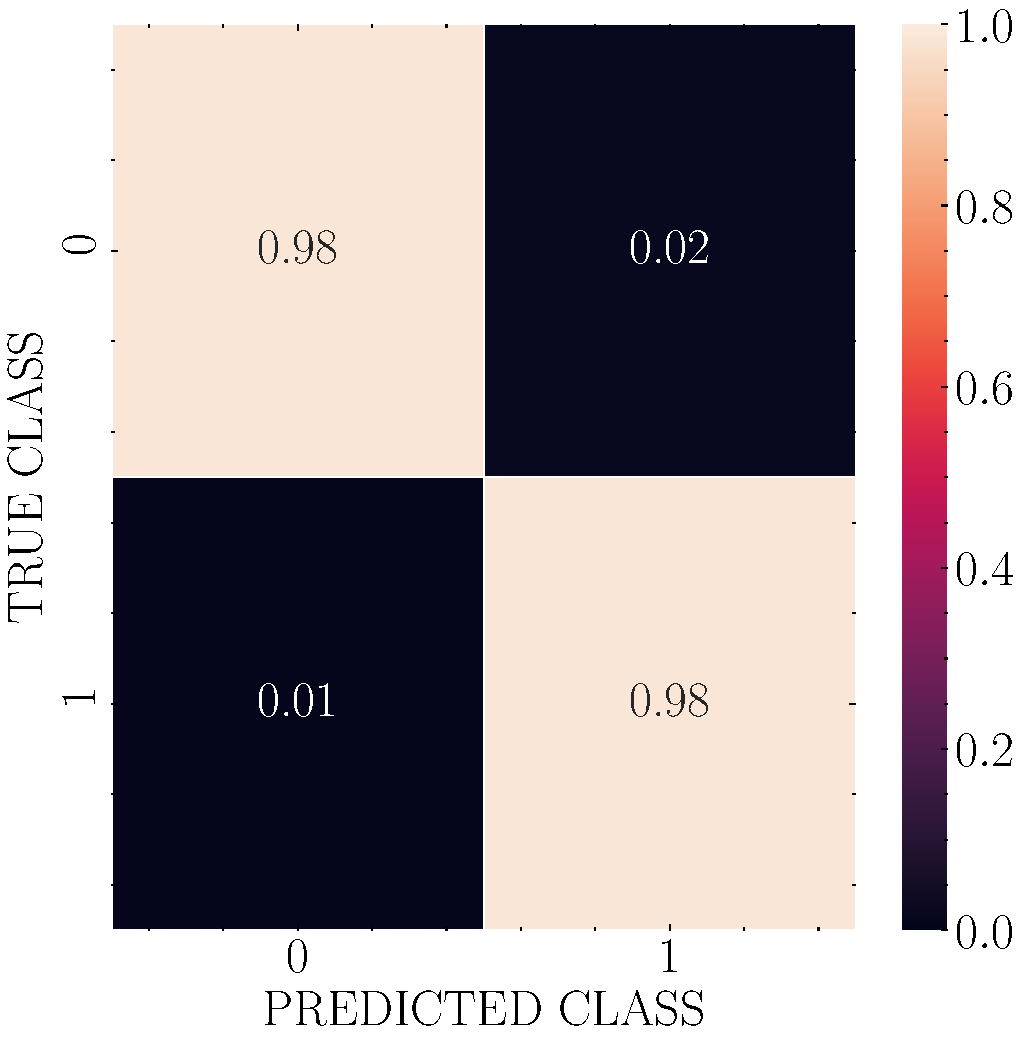
\includegraphics[width=1.5in]{../results/ex1/conf_mtx_QD_ML_dataset_P1c_size_10.pdf}
       \caption{QDA on P1c, size $10$.}
       \label{fig:QDA_P1c_10}
    \end{subfigure}
\quad
    \begin{subfigure}[!htbp]{0.24\textwidth}
       \centering
       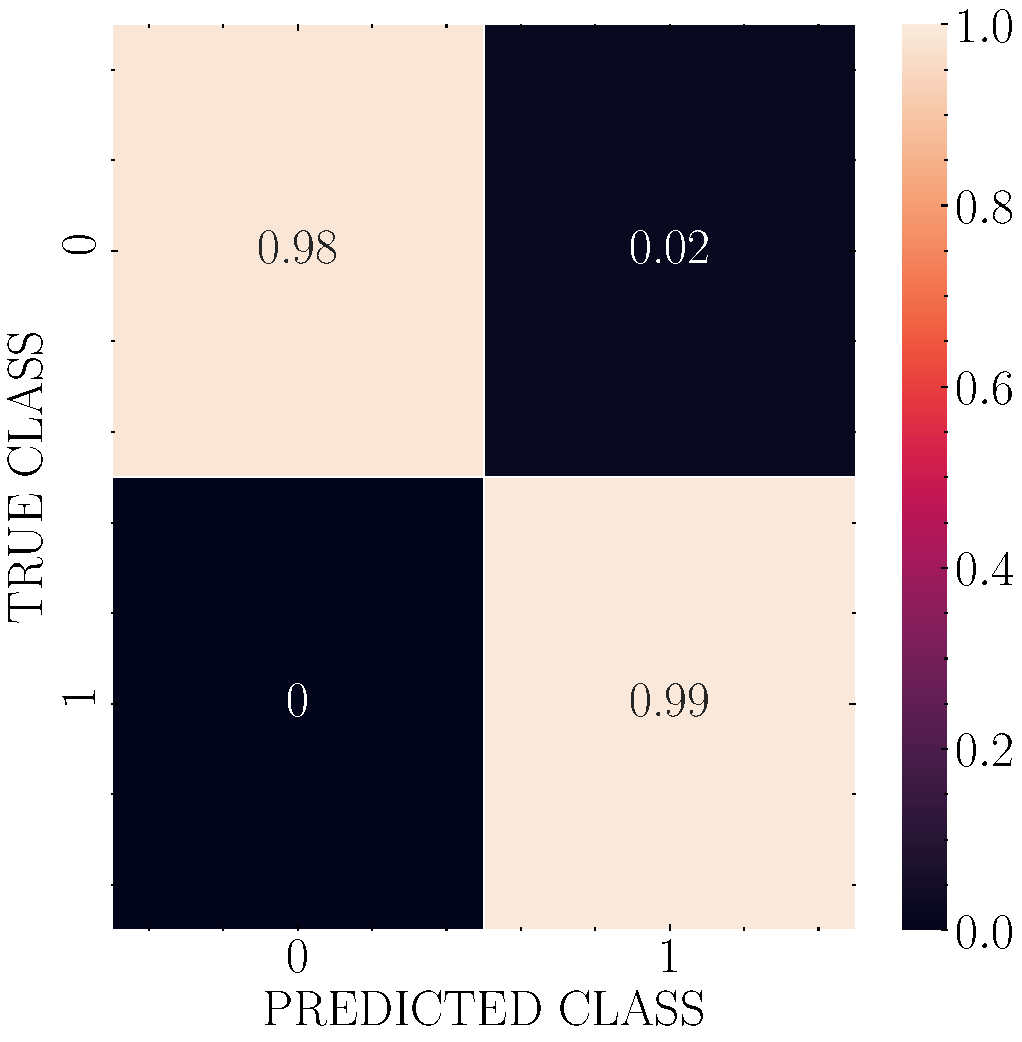
\includegraphics[width=1.5in]{../results/ex1/conf_mtx_KNN_dataset_P1c_size_10.pdf}
       \caption{KNN on P1c, size $10$.}
       \label{fig:KNN_P1c_10}
    \end{subfigure}
\quad
    \begin{subfigure}[!htbp]{0.24\textwidth}
       \centering
       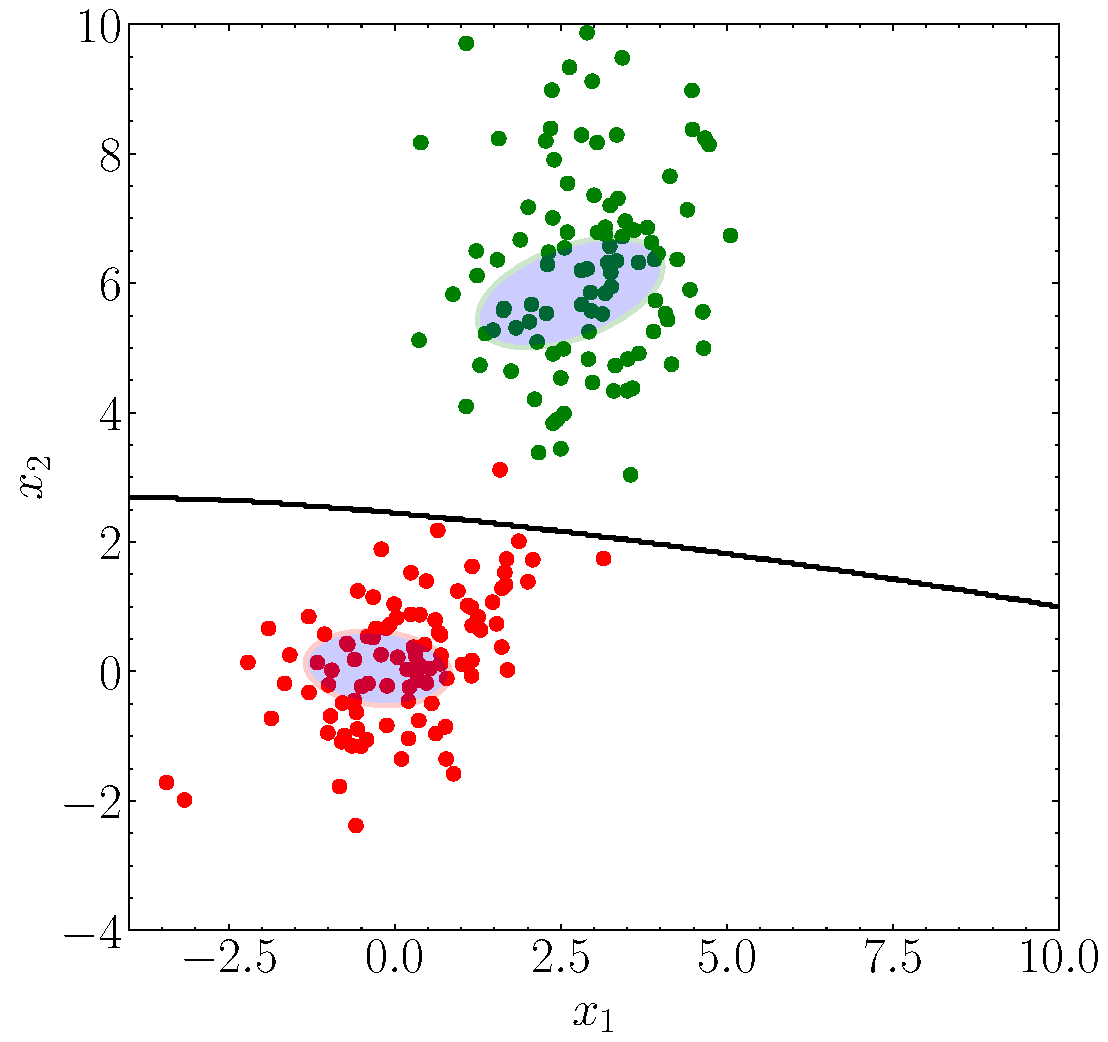
\includegraphics[width=1.5in]{../results/ex1/samples_QD_ML_dataset_P1c_size_10.pdf}
       \caption{Discriminant, size $10$.}
       \label{fig:KNN_P1c_10}
    \end{subfigure}
    
\quad    
    \begin{subfigure}[!htbp]{0.24\textwidth}
       \centering
       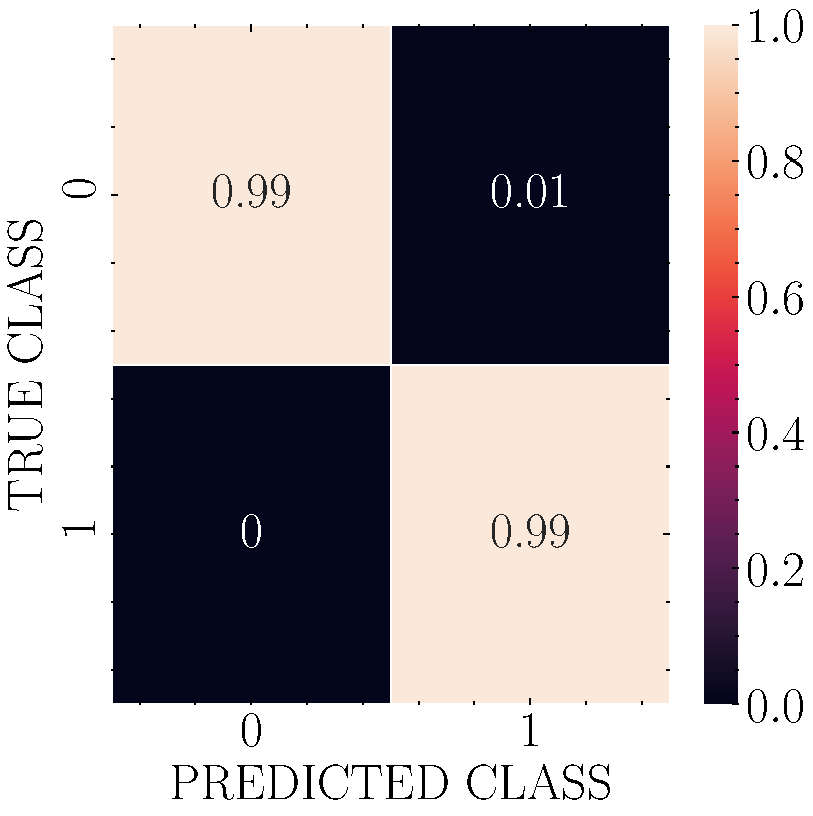
\includegraphics[width=1.5in]{../results/ex1/conf_mtx_QD_ML_dataset_P1c_size_25.pdf}
       \caption{QDA on P1c, size $25$.}
       \label{fig:KNN_P1c_25}
    \end{subfigure}
\quad    
    \begin{subfigure}[!htbp]{0.24\textwidth}
       \centering
       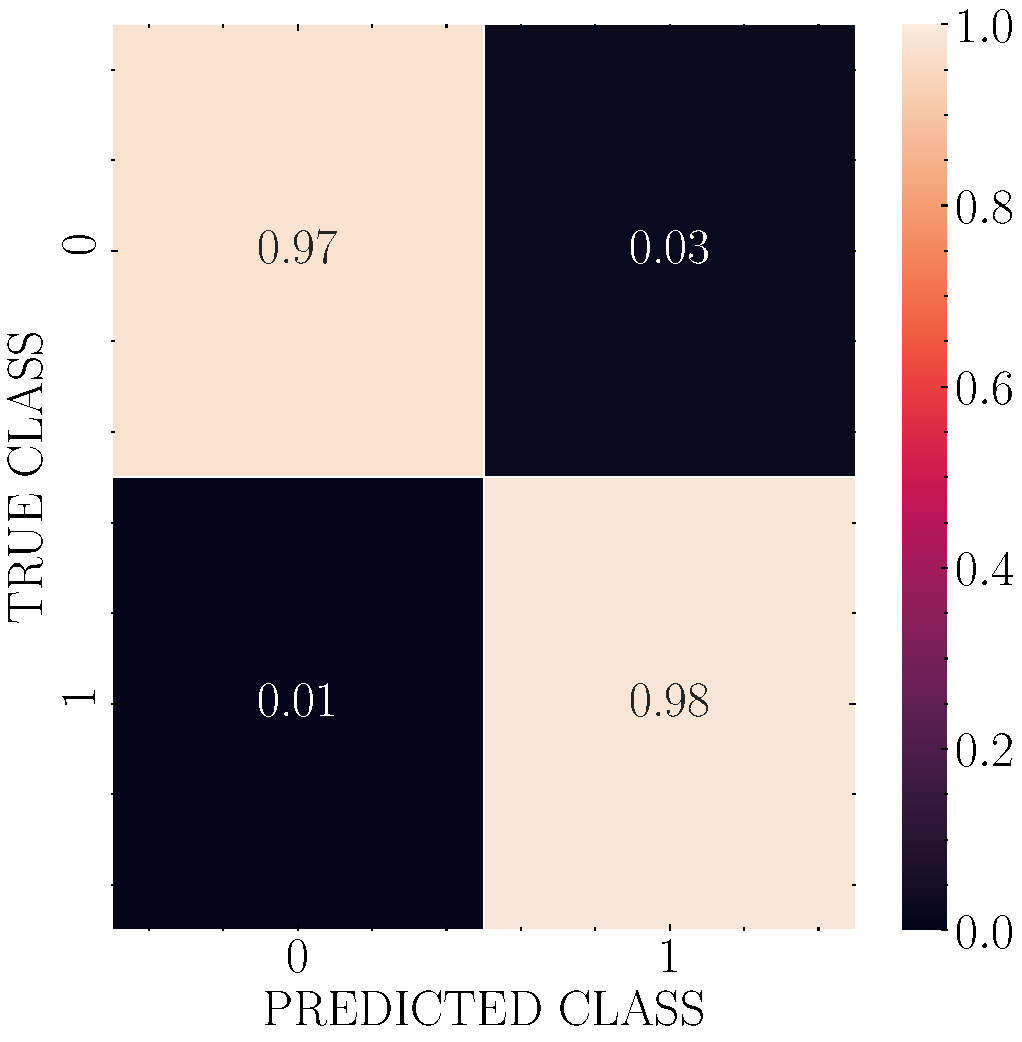
\includegraphics[width=1.5in]{../results/ex1/conf_mtx_KNN_dataset_P1c_size_25.pdf}
       \caption{KNN on P1c, size $25$.}
       \label{fig:KNN_P1c_25}
    \end{subfigure}
\quad
    \begin{subfigure}[!htbp]{0.24\textwidth}
       \centering
       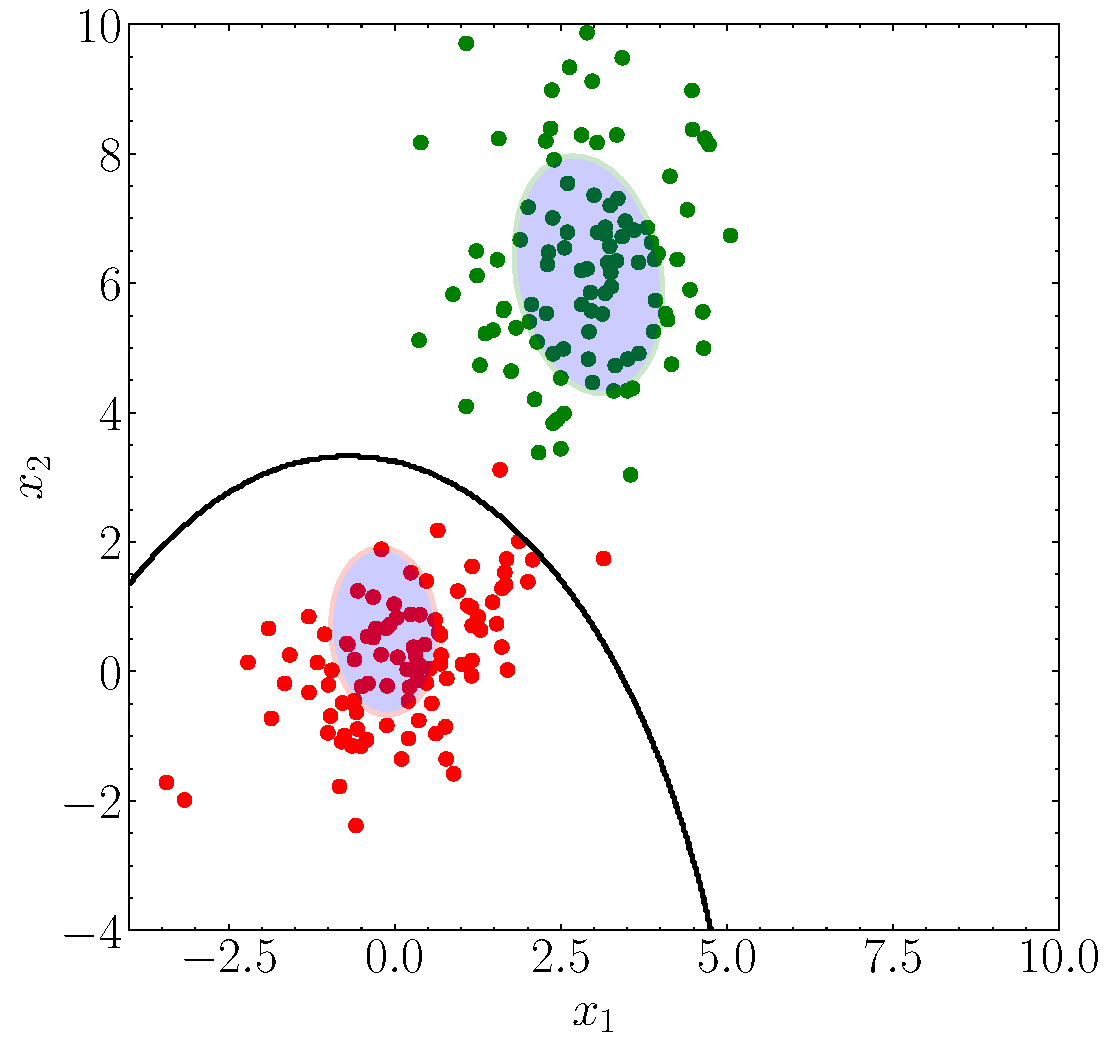
\includegraphics[width=1.5in]{../results/ex1/samples_QD_ML_dataset_P1c_size_25.pdf}
       \caption{Discriminant, size $25$.}
       \label{fig:KNN_P1c_25}
    \end{subfigure}
    
\quad    
    \begin{subfigure}[!htbp]{0.24\textwidth}
       \centering
       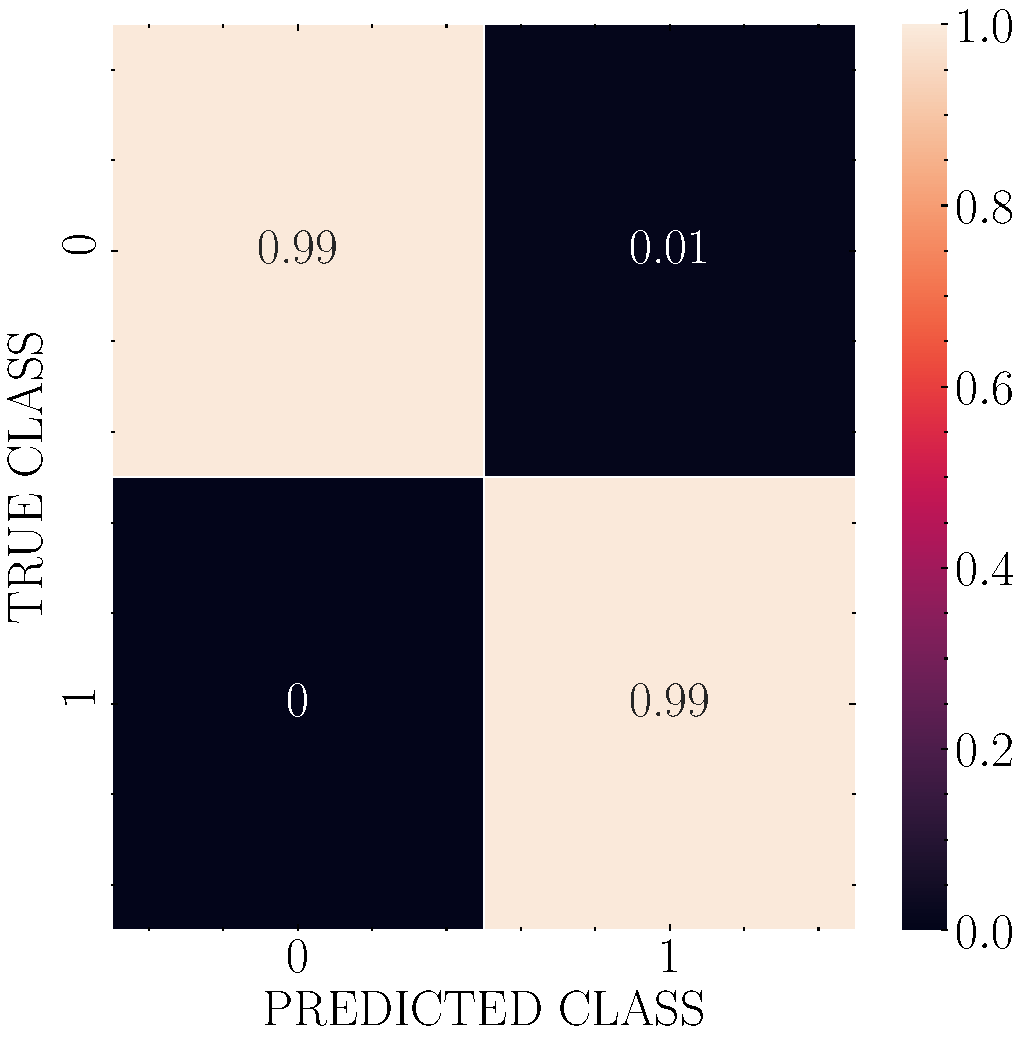
\includegraphics[width=1.5in]{../results/ex1/conf_mtx_QD_ML_dataset_P1c_size_75.pdf}
       \caption{QDA on P1c, size $75$.}
       \label{fig:KNN_P1c_75}
    \end{subfigure}
\quad    
    \begin{subfigure}[!htbp]{0.24\textwidth}
       \centering
       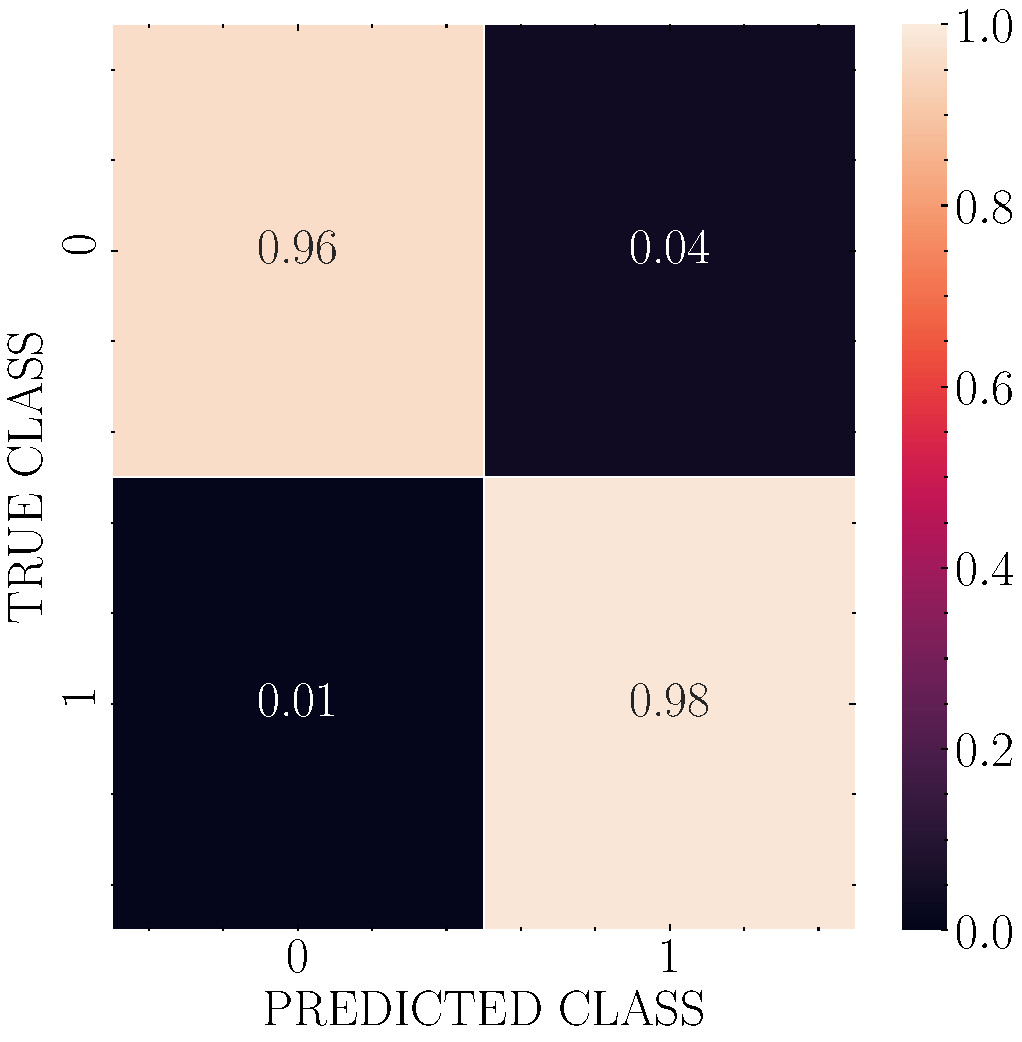
\includegraphics[width=1.5in]{../results/ex1/conf_mtx_KNN_dataset_P1c_size_75.pdf}
       \caption{KNN on P1c, size $75$.}
       \label{fig:KNN_P1c_75}
    \end{subfigure}
\quad
    \begin{subfigure}[!htbp]{0.24\textwidth}
       \centering
       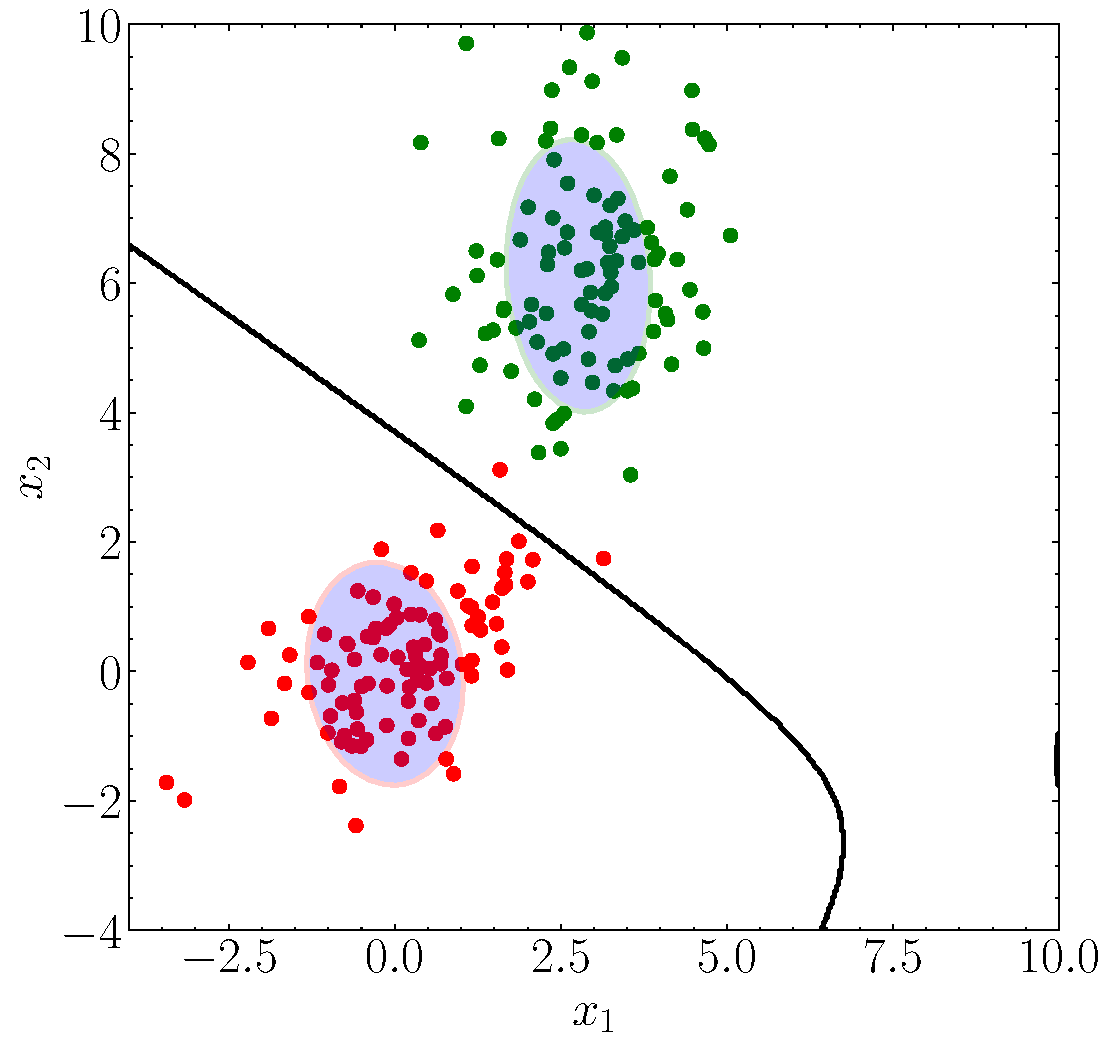
\includegraphics[width=1.5in]{../results/ex1/samples_QD_ML_dataset_P1c_size_75.pdf}
       \caption{Discriminant, size $75$.}
       \label{fig:KNN_P1c_75}
    \end{subfigure}
    
\quad    
    \begin{subfigure}[!htbp]{0.24\textwidth}
       \centering
       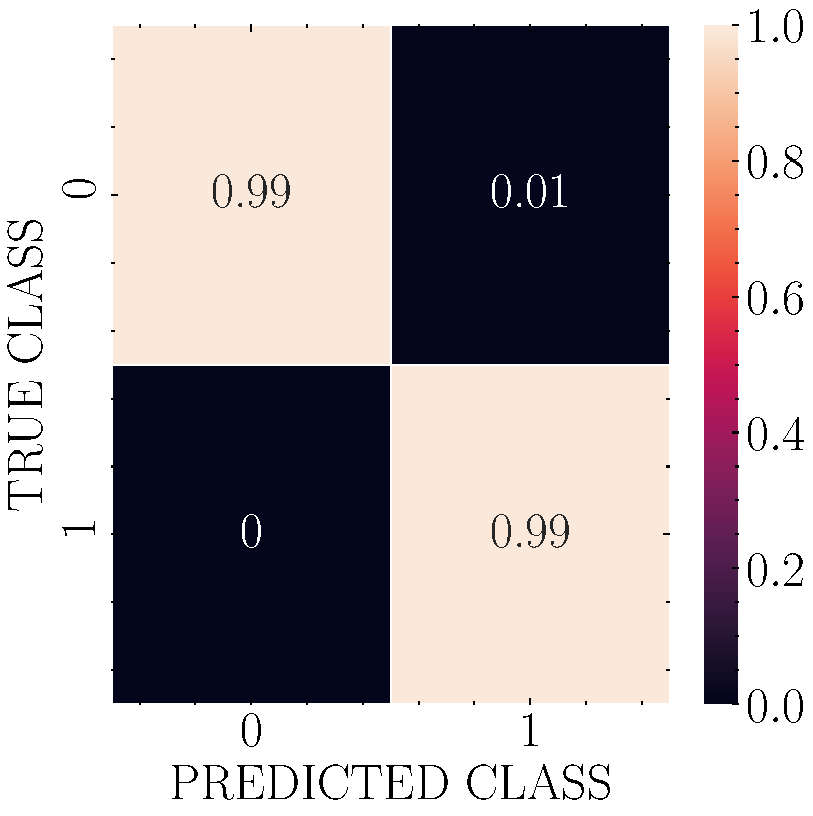
\includegraphics[width=1.5in]{../results/ex1/conf_mtx_QD_ML_dataset_P1c_size_199.pdf}
       \caption{QDA on P1c, size $199$.}
       \label{fig:KNN_P1c_199}
    \end{subfigure}
\quad    
    \begin{subfigure}[!htbp]{0.24\textwidth}
       \centering
       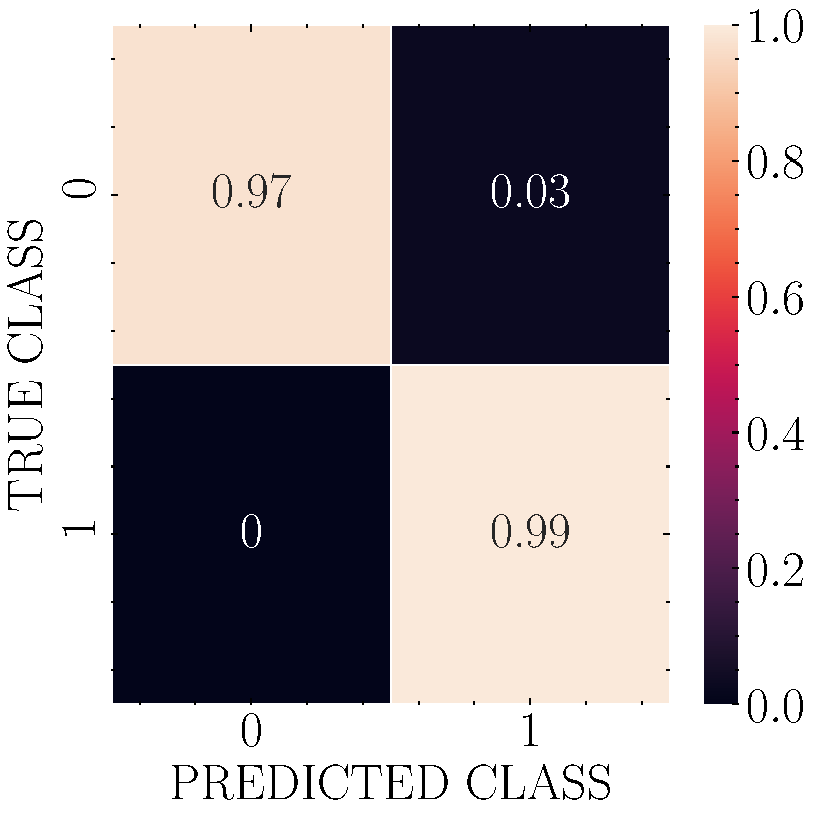
\includegraphics[width=1.5in]{../results/ex1/conf_mtx_KNN_dataset_P1c_size_199.pdf}
       \caption{KNN on P1c, size $199$.}
       \label{fig:KNN_P1c_199}
    \end{subfigure}
\quad
    \begin{subfigure}[!htbp]{0.24\textwidth}
       \centering
       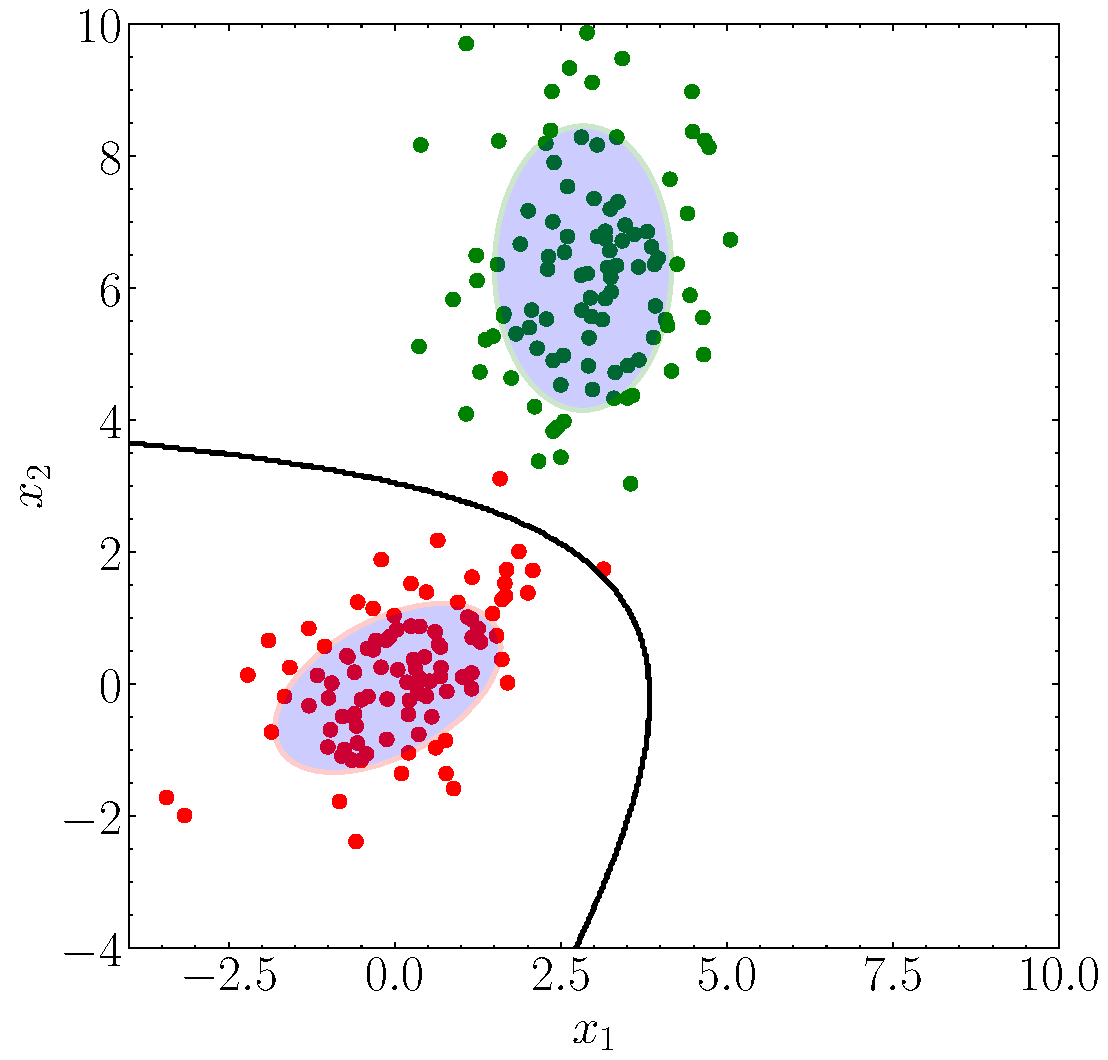
\includegraphics[width=1.5in]{../results/ex1/samples_QD_ML_dataset_P1c_size_199.pdf}
       \caption{Discriminant, size $199$.}
       \label{fig:KNN_P1c_199}
    \end{subfigure}

\caption{Bayes classifier and Nearest neighbour classification on P1c dataset.}
\label{fig:ex11P1c}
\end{figure}
{\it Inferences on P1c}: The class means are $\bmu_{0} = [0,0]^{\TT}$ and $\bmu_{1} = [3,6]^{\TT}$, and the covariances are in the same order. The class distributions are far apart, i.e., the discriminability is high. This is seen with the training samples from each class not overlapping into the other class. Within this setting, the classifiers trained with training sizes $10$, $25$, $75$, and $199$ on the average show, show an increasing trend in test accuracy. In the case where all the training samples are used, the accuracy in classification on the test data is $99\%$. When the data distributions are well separated, risk minimisation is achieved with training sample size as small as $199$ pairs. The nearest-neighbour classifier performs comparably to the Bayes' classifier. In most cases, the error in classification using nearest-neighbour classifier does not exceed twice the error in the Bayes' classifier. With increasing size of the training set, the learnt Gaussians is observed to learn ``better'', i.e., the means and covariances are closer to the true values.

% ------------------------------------------------------------------------------------------------------------------------------------------------------

\problem{Problem (1.2) Bayes' Classifier Trained using Gaussian Mixture Model}
\label{prob:1.2}


% ------------------------------------------------------------------------------------------------------------------------------------------------------

\problem{Problem (1.3) Bayes' Classifier with Exponential Class Conditional}
\label{prob:1.3}


% ------------------------------------------------------------------------------------------------------------------------------------------------------
% ------------------------------------------------------------------------------------------------------------------------------------------------------

\section{Bayes' Classifier in $\rr^{20}$}
\label{sec:bayes20D}

\problem{Problem (2) Bayes' Classifier with Gaussian Class Conditionals}
\label{prob:2}


% ------------------------------------------------------------------------------------------------------------------------------------------------------
% ------------------------------------------------------------------------------------------------------------------------------------------------------

\section{Gaussian Mixture Model in $\rr$}
\label{sec:gmm}

\problem{Problem (3) Bayes' Classifier Trained using Gaussian Mixture Model}
\label{prob:3}


% ------------------------------------------------------------------------------------------------------------------------------------------------------
% ------------------------------------------------------------------------------------------------------------------------------------------------------

\section{Naive Bayes' Classifier for Document Classification}
\label{sec:docClassification}


% ------------------------------------------------------------------------------------------------------------------------------------------------------
% ------------------------------------------------------------------------------------------------------------------------------------------------------


\end{document} 
